% ============================================================
% Capstone Project Proposal
% Improving Grasp Planning for Mobile Manipulators through
% Coordinated Base-Arm Motion Control
%
% Overleaf-ready. Compile with pdfLaTeX.
% Title page intentionally omitted.
% ============================================================

\documentclass[12pt,a4paper]{article}

\usepackage[T1]{fontenc}
\usepackage[utf8]{inputenc}
\usepackage{lmodern}
\usepackage[margin=1in]{geometry}
\usepackage{amsmath,amssymb}
\usepackage{graphicx}
\usepackage{subcaption}
\usepackage{setspace}
\usepackage{enumitem}
\usepackage{titlesec}
\usepackage[hidelinks]{hyperref}
\usepackage{xcolor}
\graphicspath{{figures/}{images/}}
\usepackage{tikz}

\bibliographystyle{plain} % or apalike for APA-like style
  

\onehalfspacing
\setlength{\parindent}{0.5in}
\setlist[itemize]{itemsep=2pt,topsep=4pt}
\setlist[enumerate]{itemsep=2pt,topsep=4pt}

\titleformat{\section}{\normalfont\large\bfseries}{\thesection}{1em}{}
\titleformat{\subsection}{\normalfont\normalsize\bfseries}{\thesubsection}{1em}{}
\titleformat{\subsubsection}{\normalfont\normalsize\itshape}{\thesubsubsection}{1em}{}

% --- Placeholder box for figures that are not yet inserted -------------
% Replace \figplaceholder{...}{...} with \includegraphics when the real
% image files are available.
% \begin{figure}
%     \centering
%     
\includegraphics[width=0.5\linewidth]{chula_logo_thumb.png}
% \end{figure}
\newcommand{\figplaceholder}[2]{%
  \fbox{\begin{minipage}[c][#2][c]{#1}
    \centering \textit{[ Image placeholder ]}
  \end{minipage}}%
}

\begin{document}

% ============================================================
% TITLE PAGE
% ============================================================
\begin{titlepage}
\centering
\thispagestyle{empty}
\vspace*{0.8in}

% ---------------- LOGO PLACEHOLDER --------------------------
% Replace the placeholder below with:
%   \includegraphics[width=0.40\textwidth]{chula_logo.png}
% \figplaceholder{0.40\textwidth}{3cm}
% \begin{figure}
%     \centering
%     
\includegraphics[width=0.5\linewidth]{chula_logo_thumb.png}
% \end{figure}

\includegraphics[width=0.40\textwidth]{chula_logo.jpg}
% ------------------------------------------------------------

\vspace{0.5in}

{\LARGE\bfseries Capstone Project Second Progress Report\par}

\vspace{0.35in}

{\large\bfseries Topic\par}
\vspace{0.10in}
{\large Improving Grasp Planning for Mobile Manipulators through\\
Coordinated Base--Arm Motion Control\par}

\vspace{0.55in}

{\large\bfseries Advisor\par}
\vspace{0.10in}
{\large Assoc.Prof. Ronnapee Chaichaowarat, Ph.D.\par}

\vspace{0.55in}

{\large\bfseries Submitted By\par}
\vspace{0.10in}
{\large
Supphakorn Akkapoo 6638226721\\
Natapol Chusang 6638050521\\
Taratorn Assawadejmetakul 6638087821\par}

\vspace{0.55in}

{\large\bfseries Majors\par}
\vspace{0.10in}
{\large Robotics and Artificial Intelligence Engineering\par}

\vfill
\end{titlepage}

\setcounter{page}{1}

% ============================================================
\section*{Inverse Kinematics Development}
\subsection*{Initial Kinematics Modeling}
Following the initial setup of the MuJoCo simulation environment as a substitute for the Walkie model, the existing \textcolor{blue}{\href{https://github.com/enactic/openarm_mujoco}{Bimanual OpenArm Mujoco Simulation}} was adapted to incorporate additional degrees of freedom representing the mobile base, including base translation, lift, and orientation control. This allows the mobile base and manipulator to be controlled as a unified system.

An initial experiment implementing inverse kinematics (IK) for coordinated base–arm motion has been conducted. This serves as a preliminary test of the proposed control approach and provides a foundation for further development of the inverse kinematics solver, motion planning, and coordinated control methods.

The whole-body system is defined by three major joint-state groups: the mobile base (4 DOF), the left arm (7 DOF), and the right arm (7 DOF).
\begin{gather*}
    \mathbf{q}_B=[\ x,\ y,\ lift,\ \psi\ ]^T\\
    \mathbf{q}_{L} = [\ q_{L_1},\ q_{L_2},\ ...,\ q_{L_7}\ ]^T\\ 
    \mathbf{q}_{R} = [\ q_{R_1},\ q_{R_2},\ ...,\ q_{R_7}\ ]^T
\end{gather*}

To simplify the initial implementation and evaluation of whole-body control, the scope is restricted to the mobile base and left arm, while the right arm is excluded from the current model. The resulting joint-state vector is defined as:
\begin{equation}
    \mathbf{q} = [\ \mathbf{q}_B;\ \mathbf{q}_L\ ]= [\ x,\ y,\ lift,\ \psi, \ q_{L_1},\ q_{L_2},\ ...,\ q_{L_7}\ ]^T \in\mathbb{R}^{11}
\end{equation}

\newpage

\subsection*{Forward Kinematics}

The forward kinematics (FK) of the left side was derived using the Standard Denavit–Hartenberg (DH) parameter. The corresponding DH parameters are summarized in Table 1 below. 

\begin{table}[htbp]
    \centering
    
    \begin{tabular}{c c c c c}
        \hline
        Link & $d$ (m) & $\theta$ (rad) & $a$ (m) & $\alpha$ (rad) \\
        \hline
        1  & 0 & $-\pi/2$ & 0 & $-\pi/2$ \\
        2  & $x^*$ & 0 & 0 & 0 \\
        3  & 0 & 0 & 0 & $\pi/2$ \\
        4  & 0 & $\pi/2$ & 0 & $-\pi/2$ \\
        5  & $y^*$ & 0 & 0 & 0 \\
        6  & 0 & 0 & 0 & $\pi/2$ \\
        7  & $\mathrm{lift}^*$ & $\mathrm{\psi }^*$ & 0 & 0 \\
        8  & 0.597 & 0 & 0 & 0 \\
        9  & 0 & 0 & 0 & $-\pi/2$ \\
        10 & 0.0915 & $q_{L_1}^*+\pi/2$ & 0 & 0 \\
        11 & 0.061131 & 0 & 0 & $-\pi/2$ \\
        12 & 0 & $q_{L_2}^*$ & 0.063 & 0 \\
        13 & 0 & $-\pi/2$ & 0 & $-\pi/2$ \\
        14 & 0.157 & $q_{L_3}^*+\pi/2$ & 0 & 0 \\
        15 & 0 & 0 & 0 & $-\pi/2$ \\
        16 & 0 & $q_{L_4}^*-\pi/2$ & 0 & 0 \\
        17 & 0 & $\pi/2$ & 0 & $\pi/2$ \\
        18 & 0.0965 & $q_{L_5}^*$ & 0 & 0 \\
        19 & 0.1195 & $-\pi/2$ & 0 & $-\pi/2$ \\
        20 & 0 & $q_{L_6}^*-\pi/2$ & 0 & 0 \\
        21 & 0 & 0 & 0 & $-\pi/2$ \\
        22 & 0 & $q_{L_7}^*$ & 0.114501 & 0 \\
        23 & 0 & $-\pi/2$ & 0 & $-\pi/2$ \\
        24 & 0 & $-\pi/2$ & 0 & 0 \\
        \hline
    \end{tabular}
    \caption{\small{Standard Denavit--Hartenberg parameters for the unified mobile base--left arm model.}}
    \label{tab:dh_parameters}
\end{table}



The forward kinematics is derived by multiplying the homogeneous transformation matrices between consecutive coordinate frames. Using the Denavit–Hartenberg (DH) convention, the transformation matrix from frame \(i-1\) to frame \(i\) is defined as:
\begin{equation}
    {}^{i-1}\mathbf{T}_{i} =
    \begin{bmatrix}
        \cos\theta_i & -\sin\theta_i\cos\alpha_i & \sin\theta_i\sin\alpha_i & a_i\cos\theta_i\\
        \sin\theta_i & \cos\theta_i\cos\alpha_i & -\cos\theta_i\sin\alpha_i & a_i\sin\theta_i\\
        0 & \sin\alpha_i & \cos\alpha_i & d_i\\
        0 & 0 & 0 & 1
    \end{bmatrix}
\end{equation}



\newpage
The overall transformation from the base frame to the end-effector frame is obtained by multiplying the individual transformation matrices along the kinematic chain:
\begin{equation}
    {}^{0}\mathbf{T}_{n}
    =
    {}^{0}\mathbf{T}_{1}
    {}^{1}\mathbf{T}_{2}
    \cdots
    {}^{n-1}\mathbf{T}_{n}
\end{equation}


\begin{figure}[htbp]
    \centering
    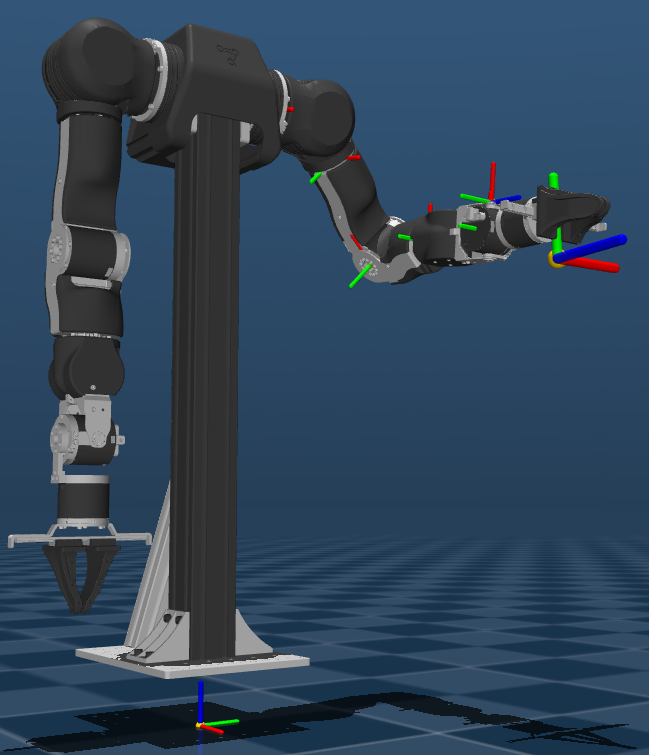
\includegraphics[scale=0.3]{joint_state_again.png}
    \caption{\small{Joint-state configuration visualized in MuJoCo
    based on the DH parameters.}}
    \label{fig:joint_state_visualized}
\end{figure}




% For the unified mobile base--left arm system, the forward kinematics
% describes the end-effector pose as a function of the joint-state
% vector $\mathbf{q}$. The end-effector pose is represented as:
% \begin{equation}
%     \mathbf{X}(\mathbf{q}) =
%     \begin{bmatrix}
%         x_e & y_e & z_e & \phi_e & \theta_e & \psi_e
%     \end{bmatrix}^{T}
% \end{equation}
% where $x_e$, $y_e$, and $z_e$ represent the end-effector position,
% while $\phi_e$, $\theta_e$, and $\psi_e$ represent its orientation
% in Euler angles.

% To establish the relationship between the joint-state vector and
% the end-effector motion, differential kinematics is employed:
% \begin{equation}
%     \begin{bmatrix}
%         \mathbf{v}_e\\
%         \boldsymbol{\omega}_e
%     \end{bmatrix}
%     =
%     \mathbf{J}(\mathbf{q})\dot{\mathbf{q}}
% \end{equation}
% where $\mathbf{v}_e \in \mathbb{R}^{3}$ and
% $\boldsymbol{\omega}_e \in \mathbb{R}^{3}$ represent the end-effector
% linear and angular velocities, respectively, and
% $\dot{\mathbf{q}} \in \mathbb{R}^{11}$ is the joint-velocity vector
% of the mobile base and left arm. The geometric Jacobian
% $\mathbf{J}(\mathbf{q}) \in \mathbb{R}^{6 \times 11}$ is defined as:
% \begin{equation}
%     \mathbf{J}(\mathbf{q}) =
%     \begin{bmatrix}
%         \mathbf{J}_v(\mathbf{q})\\
%         \mathbf{J}_{\omega}(\mathbf{q})
%     \end{bmatrix}
% \end{equation}
% where $\mathbf{J}_v$ and $\mathbf{J}_{\omega}$ map the joint
% velocities to the end-effector linear and angular velocities,
% respectively. Each column describes the contribution of an individual
% joint variable to the end-effector motion. By incorporating both the
% mobile base and manipulator degrees of freedom, the Jacobian provides
% the differential kinematic model required for coordinated base--arm
% inverse kinematics.


For the initial implementation, the forward kinematics (FK) only maps
the joint-state vector $\mathbf{q}$ to the end-effector position
in Cartesian space. The end-effector position is expressed as:
\begin{equation}
    \mathbf{p}(\mathbf{q}) =
    \begin{bmatrix}
        x_e & y_e & z_e
    \end{bmatrix}^{T}
\end{equation}
where $x_e$, $y_e$, and $z_e$ represent the end-effector position
along the $x$, $y$, and $z$ axes, respectively — obtained from the transformation matrix.

The relationship between joint motion and end-effector motion is
described by differential kinematics:
\begin{equation}
    \dot{\mathbf{p}} =
    \mathbf{J}(\mathbf{q})\dot{\mathbf{q}}
\end{equation}
where $\dot{\mathbf{p}} \in \mathbb{R}^{3}$ represents the
end-effector linear velocity, $\dot{\mathbf{q}}$ is the
joint-velocity vector, and $\mathbf{J}(\mathbf{q})$ is the
position Jacobian, which maps joint velocities to end-effector linear velocity. 
\newpage

% \subsection*{Jacobian Pseudoinverse}
% From differential kinematics, we can rearrangement the equation as:

% \begin{equation}
%     \mathbf{\dot q}=\mathbf{J(q) }^{-1}\mathbf{\dot p} 
% \end{equation}

% Often times, in these problems, the $\mathbf{J(q)}$ is either a non-full rank or non-singular matrix, leading to failure in matrix inversion. Therefore a Moore-Penrose Pseudoinverse is used instead, where

% \begin{equation}
%     A^{\dagger} = (AA^T)^{-1}A^T
% \end{equation}

% denoted by the $\mathbf{\dagger}$ expression, therefore the equation thus become:

% \begin{equation}
%     \mathbf{\dot q}=\mathbf{J(q) }^{\dagger}\mathbf{\dot p}
% \end{equation}

% This established the foundation for subsequent inverse kinematics development.


\subsection*{Jacobian Pseudoinverse}

From differential kinematics, the relationship between joint
velocities and end-effector velocity is given by:
\begin{equation}
    \dot{\mathbf{p}} = \mathbf{J}(\mathbf{q})\dot{\mathbf{q}}
\end{equation}

To obtain the joint velocities required to achieve a desired
end-effector velocity, the equation can be solved using the
inverse of the Jacobian when the matrix is square and invertible.
However, in redundant robotic systems, the Jacobian is generally
non-square, and it may also become rank-deficient near kinematic
singularities. Consequently, directly inverting the Jacobian is
not generally applicable.

To address this, the Moore--Penrose pseudoinverse is used to compute a least-squares solution~\cite{buss2009}. For a matrix $\mathbf{A}$ with
full row rank, its pseudoinverse is given by:
\begin{equation}
    \mathbf{A}^{\dagger}
    = \mathbf{A}^{T}
    \left(\mathbf{A}\mathbf{A}^{T}\right)^{-1}
\end{equation}

Applying the pseudoinverse to the position Jacobian gives:
\begin{equation}
    \dot{\mathbf{q}}
    = \mathbf{J}(\mathbf{q})^{\dagger}\dot{\mathbf{p}}
\end{equation}

To apply this formulation to iterative inverse kinematics, the
end-effector velocity $\dot{\mathbf{p}}$ is replaced with the
Cartesian position error:
\begin{equation}
    \mathbf{e} =
    \mathbf{p}_{\mathrm{target}} -
    \mathbf{p}(\mathbf{q}_k)
\end{equation}
The resulting joint-state update is approximated numerically as:
\begin{equation}
    \Delta\mathbf{q}
    = \mathbf{J}(\mathbf{q}_k)^{\dagger}\mathbf{e},
    \qquad
    \mathbf{q}_{k+1}
    = \mathbf{q}_k + \Delta\mathbf{q}
\end{equation}
where $\mathbf{q}_k$ represents the joint-state vector at iteration
$k$, and $\Delta\mathbf{q}$ is the calculated joint-state update.
The process is repeated until the end-effector position error
falls below a specified tolerance.

This approach provides a computationally efficient method for
iteratively reducing Cartesian position error and demonstrated
rapid convergence in the initial inverse kinematics implementation.
However, near kinematic singularities, the pseudoinverse can
produce excessively large joint-state updates, motivating the subsequent adoption of the damped least squares method.
\newpage


\subsection*{Damped Least Squares (DLS)}
As the end-effector approaches a kinematic singularity, the
Jacobian pseudoinverse may produce excessively large joint-state
updates, resulting in unstable motion. To address this limitation,
the Damped Least Squares (DLS) method~\cite{buss2009} introduces a damping term
into the pseudoinverse formulation, improving numerical stability
while limiting the magnitude of the joint-state updates.

Using the Jacobian $\mathbf{J}$ and the end-effector position error
$\mathbf{e}$, the conventional pseudoinverse solution is:
\begin{equation}
    \Delta\mathbf{q} = \mathbf{J}^{\dagger}\mathbf{e}
\end{equation}
This solution minimizes the joint update norm among all
least-squares solutions:
\begin{equation}
    \min_{\Delta\mathbf{q}} \|\Delta\mathbf{q}\|^2
\end{equation}
subject to minimizing the Cartesian error:
\begin{equation}
    \min_{\Delta\mathbf{q}}
    \|\mathbf{e}-\mathbf{J}\Delta\mathbf{q}\|^2
\end{equation}
where $\|\cdot\|$ denotes the Euclidean norm. When an exact
solution exists, the pseudoinverse provides the minimum-norm
joint update that achieves the desired Cartesian displacement.

The DLS method introduces a damping factor to regularize this
optimization problem. Its damped pseudoinverse is defined as:
\begin{equation}
    \mathbf{J}^{\#}
    =
    \mathbf{J}^{T}
    \left(
        \mathbf{J}\mathbf{J}^{T}
        + \lambda^2\mathbf{I}
    \right)^{-1},
    \qquad \lambda > 0
\end{equation}
where $\lambda$ is the damping factor and $\mathbf{I}$ is the
identity matrix. The resulting joint update is:
\begin{equation}
    \Delta\mathbf{q} = \mathbf{J}^{\#}\mathbf{e}
\end{equation}

This formulation is equivalent to minimizing the following
regularized least-squares objective:
\begin{equation}
    \min_{\Delta\mathbf{q}}
    \left\{
        \|\mathbf{e}-\mathbf{J}\Delta\mathbf{q}\|^2
        + \lambda^2\|\Delta\mathbf{q}\|^2
    \right\}
\end{equation}
The first term minimizes the Cartesian position error, while
the second penalizes large joint-state updates. Consequently,
DLS improves numerical stability near singularities by
regularizing the solution and limiting excessively large updates. 
\newpage

The effect of the damping near a singularity is shown in the
\textcolor{blue}{\href{https://youtu.be/MEW62I4-9JQ}{comparison video}}, in which the same target is solved with the plain pseudoinverse (Fig.~\ref{fig:dls_comparison}a) and with DLS (Fig.~\ref{fig:dls_comparison}b). Near the singular
configuration the pseudoinverse produces large joint-state updates and
unstable motion, whereas DLS keeps the updates bounded and the motion
smooth, at the cost of a slightly slower approach to the target.

\begin{figure}[htbp]
    \centering
    \begin{subfigure}[t]{0.48\textwidth}
        \centering
        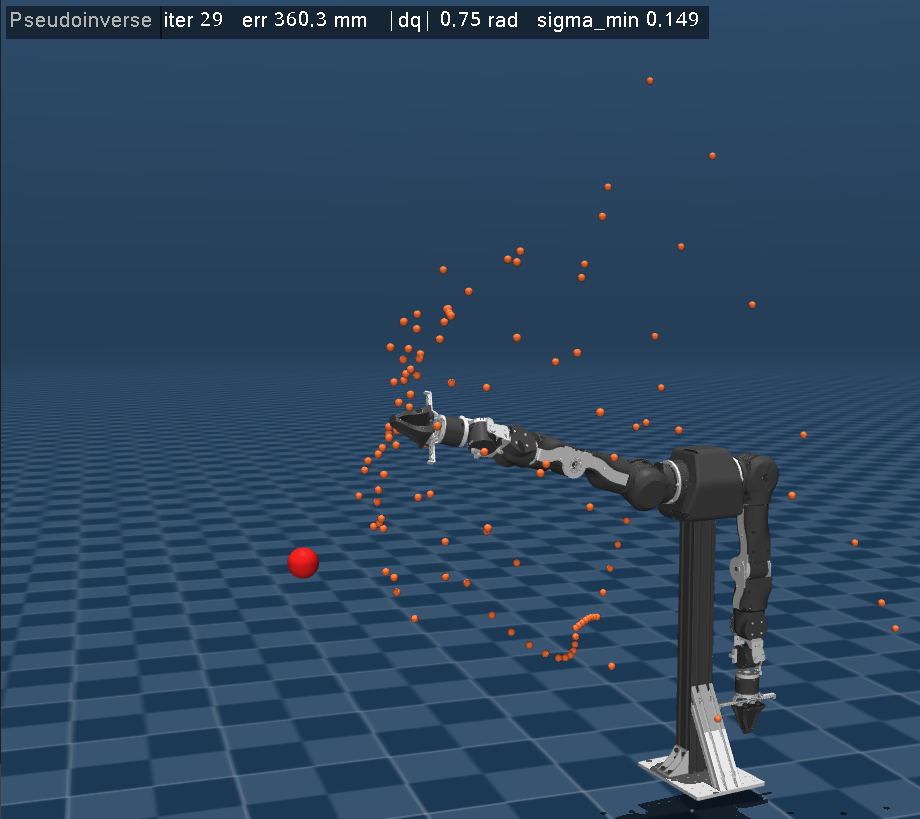
\includegraphics[height=7cm]{pinv_singularity.png}
        \caption{Pseudoinverse (no damping)}
    \end{subfigure}\hfill
    \begin{subfigure}[t]{0.48\textwidth}
        \centering
        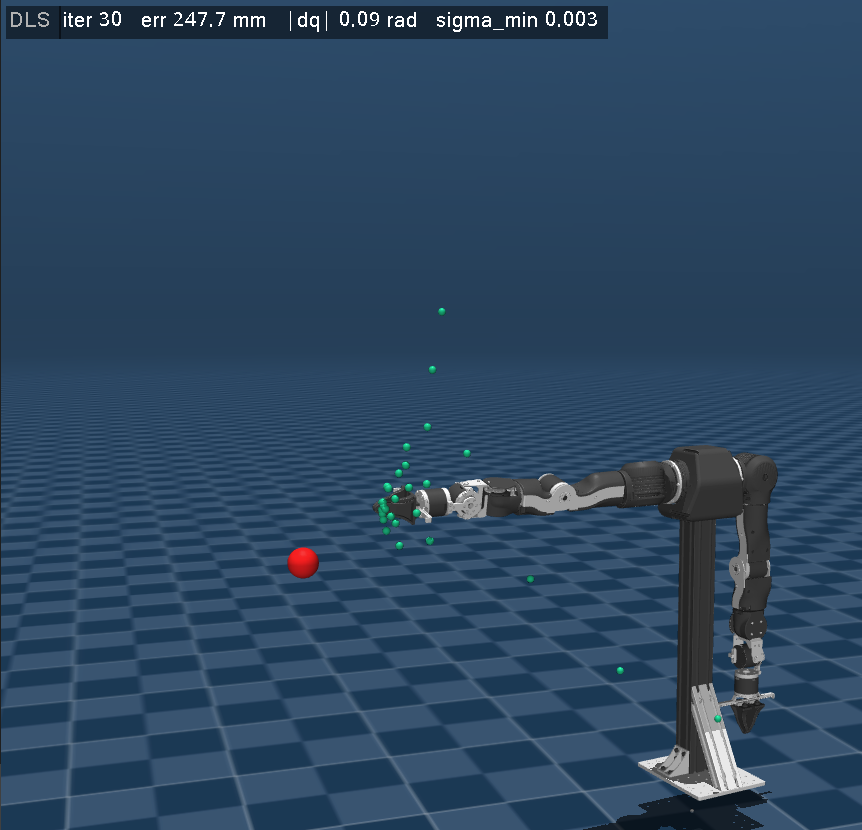
\includegraphics[height=7cm]{dls_singularity.png}
        \caption{Damped least squares}
    \end{subfigure}
    \caption{\small{Frames from the comparison video near a singular
    configuration, using the same target (red sphere) and initial state. Each small dot represent the end-effector position solved by each iteration.}} 
    \label{fig:dls_comparison}
\end{figure}


The improvement in stability can be seen in the comparison
video, where the same target is solved with
the conventional pseudoinverse and with DLS. Near the singular
configuration, the pseudoinverse produced large joint-state updates and unstable motion, whereas DLS kept the updates bounded and the motion smooth. This stability came at the cost of slower convergence toward the target, which motivated further development of the inverse kinematics
solver.
\newpage

\subsection*{Per-Joint Weighted Damping}
The scalar damping factor $\lambda$ in the DLS formulation penalizes the motion of every joint equally. For the unified base--arm system this is a poor fit: the base joints $x$, $y$, and $lift$ are prismatic (meters) while the arm joints are revolute (radians), so a single $\lambda$ cannot express how willing each joint should be to move. To give every joint its own cost of motion, the damping is generalized to a diagonal matrix, following the dynamic weighting of damped least squares in~\cite{schinstock1994}:
\begin{equation}
    \boldsymbol{\Lambda} = \operatorname{diag}\!\left(\lambda_1^2,\ \lambda_2^2,\ \dots,\ \lambda_n^2\right),
    \qquad n = 11
\end{equation}
and the DLS objective becomes
\begin{equation}
    \min_{\Delta\mathbf{q}}
    \left\{
        \|\mathbf{e}-\mathbf{J}\Delta\mathbf{q}\|^2
        + \Delta\mathbf{q}^{T}\boldsymbol{\Lambda}\,\Delta\mathbf{q}
    \right\}
\end{equation}
Setting the gradient with respect to $\Delta\mathbf{q}$ to zero gives the normal equations:
\begin{equation}
    \left(\mathbf{J}^{T}\mathbf{J} + \boldsymbol{\Lambda}\right)\Delta\mathbf{q}
    = \mathbf{J}^{T}\mathbf{e}
    \label{eq:weighted_dls}
\end{equation}
A larger $\lambda_i$ makes joint $i$ more expensive to move, shifting the update onto the remaining joints. Because $\boldsymbol{\Lambda}$ is $n\times n$, the system is solved in joint space ($11\times 11$) rather than in task space ($3\times 3$). For $\boldsymbol{\Lambda}=\lambda^2\mathbf{I}$ it reduces to the DLS update of the previous section, since $(\mathbf{J}^{T}\mathbf{J}+\lambda^2\mathbf{I})^{-1}\mathbf{J}^{T} = \mathbf{J}^{T}(\mathbf{J}\mathbf{J}^{T}+\lambda^2\mathbf{I})^{-1}$.

\newpage
\subsection*{Joint-Limit Damping}
Hard clipping alone lets a joint run into its limit and then stall. Instead, the damping of a joint is increased only when that joint is moving \emph{toward} its nearest limit. For a joint with finite range $[q_i^{\min},\,q_i^{\max}]$, the normalized distance to the limit it is heading toward is
\begin{equation}
    d_i =
    \begin{cases}
        \dfrac{q_i^{\max}-q_i}{q_i^{\max}-q_i^{\min}}, & \Delta q_i \ge 0\\[2ex]
        \dfrac{q_i-q_i^{\min}}{q_i^{\max}-q_i^{\min}}, & \Delta q_i < 0
    \end{cases}
\end{equation}
Let $m$ be the width of the margin zone, expressed as a fraction of the joint range, so that the zone at each end of the range is $m\,(q_i^{\max}-q_i^{\min})$ wide (Fig.~\ref{fig:margin_zone}). The penetration into this zone and the resulting weight are
\begin{equation}
    p_i = \operatorname{clip}\!\left(\frac{m-d_i}{m},\ 0,\ 1\right),
    \qquad
    w_i = 1 + g\,\frac{p_i^{2}}{1-p_i+\varepsilon}
    \label{eq:limit_weight}
\end{equation}

where $g$ is the penalty gain and $\varepsilon$, an extremely small constant ($\leq 0.001$), to prevent division by zero. The weights enter the damping as $\boldsymbol{\Lambda}\mathbf{W}$, with $\mathbf{W}=\operatorname{diag}(w_i)$:
\begin{equation}
    \Delta\mathbf{q}
    = \left(\mathbf{J}^{T}\mathbf{J} + \boldsymbol{\Lambda}\mathbf{W}\right)^{-1}\mathbf{J}^{T}\mathbf{e}
\end{equation}

\begin{figure}[htbp]
    \centering
    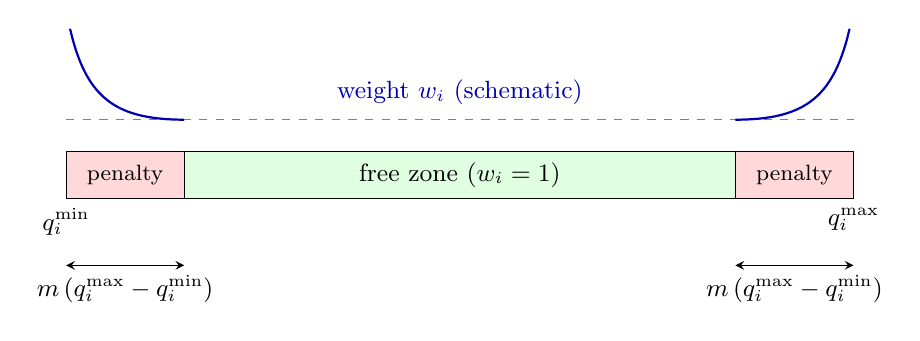
\begin{tikzpicture}[>=stealth, font=\small]
        % joint range split into penalty / free / penalty zones (m = 0.15 drawn to scale)
        \fill[red!15]   (0,0)   rectangle (1.5,0.6);
        \fill[green!12] (1.5,0) rectangle (8.5,0.6);
        \fill[red!15]   (8.5,0) rectangle (10,0.6);
        \draw (0,0) rectangle (10,0.6);
        \draw (1.5,0) -- (1.5,0.6);
        \draw (8.5,0) -- (8.5,0.6);
        \node at (0.75,0.3) {\footnotesize penalty};
        \node at (5,0.3)    {free zone ($w_i=1$)};
        \node at (9.25,0.3) {\footnotesize penalty};
        % joint limits
        \node[below] at (0,0)  {$q_i^{\min}$};
        \node[below] at (10,0) {$q_i^{\max}$};
        % zone widths
        \draw[<->] (0,-0.85)   -- (1.5,-0.85);
        \draw[<->] (8.5,-0.85) -- (10,-0.85);
         \node[below] at (0.75,-0.85) {$m\,(q_i^{\max}-q_i^{\min})$};
        \node[below] at (9.25,-0.85) {$m\,(q_i^{\max}-q_i^{\min})$};
        % schematic weight profile above the bar
        \draw[dashed, gray] (0,1.0) -- (10,1.0);
        \draw[thick, blue!70!black, domain=0.05:1.5, samples=40, smooth, variable=\x]
            plot ({\x},{1+0.35*((1.5-\x)/1.5)^2/(1-(1.5-\x)/1.5+0.25)});
        \draw[thick, blue!70!black, domain=0.05:1.5, samples=40, smooth, variable=\x]
            plot ({10-\x},{1+0.35*((1.5-\x)/1.5)^2/(1-(1.5-\x)/1.5+0.25)});
        \node[blue!70!black] at (5,1.35) {weight $w_i$ (schematic)};
    \end{tikzpicture}
    \caption{\small{Margin zone of a joint with limits $[q_i^{\min},q_i^{\max}]$, drawn for $m=0.15$. The weight $w_i$ equals 1 in the free zone and rises steeply toward the limit the joint is approaching.}}
    \label{fig:margin_zone}
\end{figure}
Here $w_i=1$ when the joint is outside the margin zone or moving away from the limit, so its behavior is unchanged. Inside the zone, $w_i$ grows smoothly and reaches approximately $1+g/\varepsilon$ at the limit, effectively freezing the joint. Joints without finite limits keep $w_i=1$.

Weighting the damping per joint to handle joint limits follows the dynamic-weighting idea of Schinstock et al.~\cite{schinstock1994}. It differs from selectively damped least squares~\cite{bussKim2004}, which clamps the step along each singular vector of the Jacobian rather than per joint.

\newpage
Since $w_i$ depends on the sign of $\Delta q_i$, which in turn depends on $w_i$, the system is solved by fixed-point refinement: $\Delta\mathbf{q}$ is first computed with $\mathbf{W}=\mathbf{I}$, the weights are recomputed from that step, and the system is re-solved. This is repeated $n_r$ times. Finally, the update is clipped so that no joint steps past a hard limit:
\begin{equation}
    \mathbf{q}_{k+1} = \operatorname{clip}\!\left(\mathbf{q}_k + \Delta\mathbf{q},\ \mathbf{q}^{\min},\ \mathbf{q}^{\max}\right)
\end{equation}


\subsection*{Resting-Position Pull}
With 11 degrees of freedom and a 3-dimensional position task, infinitely many joint configurations reach the same target. The damped least-squares solution selects the one with the smallest weighted step, but it does not care where inside its range each joint ends up, so repeated updates can drift the arm into awkward postures. To keep the arm in a comfortable posture while it tracks the target, each arm joint may be assigned a resting position $q_i^{\mathrm{rest}}$, and a soft cost penalizes joints that end up away from it.

Let $r_i \ge 0$ be the pull weight of joint $i$, with $r_i=0$ for joints that have no resting position (the base joints in this work). The offset from rest at iteration $k$ is
\begin{equation}
    \delta_i = q_i - q_i^{\mathrm{rest}}
\end{equation}
with $\delta_i=0$ where no resting position is defined, and $\mathbf{R}=\operatorname{diag}(r_i)$. The rest pull is added to the weighted DLS objective as a cost on the joint position \emph{after} the update, $q_i+\Delta q_i-q_i^{\mathrm{rest}}=\delta_i+\Delta q_i$:
\begin{equation}
    \min_{\Delta\mathbf{q}}
    \left\{
        \|\mathbf{e}-\mathbf{J}\Delta\mathbf{q}\|^2
        + \Delta\mathbf{q}^{T}\boldsymbol{\Lambda}\mathbf{W}\,\Delta\mathbf{q}
        + \left(\Delta\mathbf{q}+\boldsymbol{\delta}\right)^{T}\mathbf{R}\left(\Delta\mathbf{q}+\boldsymbol{\delta}\right)
    \right\}
    \label{eq:rest_objective}
\end{equation}
The first term reduces the Cartesian error, the second damps the update (with extra damping near joint limits), and the third rewards motion toward the resting position and penalizes motion away from it. Setting the gradient to zero gives
\begin{equation}
    \left(\mathbf{J}^{T}\mathbf{J} + \boldsymbol{\Lambda}\mathbf{W} + \mathbf{R}\right)\Delta\mathbf{q}
    = \mathbf{J}^{T}\mathbf{e} - \mathbf{R}\boldsymbol{\delta}
    \label{eq:rest_normal}
\end{equation}
Compared with the weighted DLS, there are two changes: $\mathbf{R}$ on the left adds damping to the joints that have a resting position, and $-\mathbf{R}\boldsymbol{\delta}$ on the right acts as a spring force, proportional to the offset and directed toward the resting position.

To see the structure of the update, define $\mathbf{M}=\boldsymbol{\Lambda}\mathbf{W}+\mathbf{R}$ and the generalized damped pseudoinverse
\begin{equation}
    \mathbf{J}^{\#}
    = \left(\mathbf{J}^{T}\mathbf{J}+\mathbf{M}\right)^{-1}\mathbf{J}^{T}
    = \mathbf{M}^{-1}\mathbf{J}^{T}\left(\mathbf{J}\mathbf{M}^{-1}\mathbf{J}^{T}+\mathbf{I}\right)^{-1}
\end{equation}
\newpage
which reduces to the DLS pseudoinverse when $\mathbf{M}=\lambda^2\mathbf{I}$. The update then decomposes as
\begin{equation}
    \Delta\mathbf{q}
    = \underbrace{\mathbf{J}^{\#}\mathbf{e}}_{\text{task term}}
    \;-\;
    \underbrace{\left(\mathbf{I}-\mathbf{J}^{\#}\mathbf{J}\right)\mathbf{M}^{-1}\mathbf{R}\,\boldsymbol{\delta}}_{\text{posture term}}
    \label{eq:rest_decomposition}
\end{equation}
The task term is the damped step toward the target. The posture term is a correction toward the resting configuration, filtered by $(\mathbf{I}-\mathbf{J}^{\#}\mathbf{J})$, the damped counterpart of the classical null-space projector $(\mathbf{I}-\mathbf{J}^{\dagger}\mathbf{J})$~\cite{schinstock1994}. Neglecting the coupling through $\mathbf{J}^{T}\mathbf{J}$, an individual joint recovers a fraction
\begin{equation}
    \frac{\Delta q_i}{-\delta_i} = \frac{r_i}{\lambda_i^2 w_i + r_i}
\end{equation}
of its offset per iteration, so a larger $r_i$ relative to the damping pulls the joint back faster, and the pull is slowed automatically near joint limits where $w_i$ is large.

The iteration converges when $\Delta\mathbf{q}=\mathbf{0}$, which by \eqref{eq:rest_normal} requires
\begin{equation}
    \mathbf{J}^{T}\mathbf{e} = \mathbf{R}\boldsymbol{\delta}
\end{equation}
The damping terms $\boldsymbol{\Lambda}\mathbf{W}$ multiply $\Delta\mathbf{q}$ and therefore vanish at convergence: they change how fast the solver converges but not where. The rest pull does shift the equilibrium, since it balances a small residual position error against the posture offset. The residual grows with $r_i$, so the pull weight is kept small relative to the Jacobian entries. This is the trade-off between posture quality and positioning accuracy that the weight $r_i$ controls.



\newpage
\subsection*{Single-Arm Implementation and Results}
Each iteration of the single-arm solver (mobile base and left arm, $n=11$) proceeds as follows:
\begin{enumerate}
    \item Compute the position error $\mathbf{e}=\mathbf{p}_{\mathrm{target}}-\mathbf{p}(\mathbf{q}_k)$ and the Jacobian $\mathbf{J}(\mathbf{q}_k)$, and form the offset $\boldsymbol{\delta}$ from the resting positions.
    \item Solve \eqref{eq:rest_normal} with $\mathbf{W}=\mathbf{I}$ to obtain a first estimate of $\Delta\mathbf{q}$.
    \item Recompute $\mathbf{W}$ from \eqref{eq:limit_weight} using this estimate and re-solve; repeat $n_r$ times.
    \item Clip $\mathbf{q}_k+\Delta\mathbf{q}$ to the joint limits to obtain $\mathbf{q}_{k+1}$.
    \item Stop when $\|\mathbf{e}\|$ falls below the position tolerance; otherwise return to step 1.
\end{enumerate}

\begin{table}[htbp]
    \centering
    \begin{tabular}{l l}
        \hline
        Parameter & Value \\
        \hline
        Damping factor $\lambda_i$ (base joints: $x$, $y$, yaw, lift) & 0.6 \\
        Damping factor $\lambda_i$ (arm joints $q_{L_1}$--$q_{L_7}$) & 0.2 \\
        Limit margin $m$ & 0.15 \\
        Limit penalty gain $g$ & 50 \\
        Refinement passes $n_r$ & 2 \\
        Rest-pull weight $r_i$ (arm joints) & 0.004 \\
        Position tolerance & $10^{-3}$ m \\
        Maximum iterations & 100 \\
        \hline
    \end{tabular}
    \caption{\small{Solver parameters used in the single-arm experiments.}}
    \label{tab:single_arm_params}
\end{table}

\begin{table}[htbp]
    \centering
    \begin{tabular}{c c c c c c c c}
        \hline
        Joint & $q_{L_1}$ & $q_{L_2}$ & $q_{L_3}$ & $q_{L_4}$ & $q_{L_5}$ & $q_{L_6}$ & $q_{L_7}$ \\
        \hline
        $q^{\mathrm{rest}}$ (rad) & 0 & $-0.4$ & 0.2 & 1.7 & 0.06 & 0 & 0 \\
        \hline
    \end{tabular}
    \caption{\small{Resting positions of the left-arm joints. The base joints have no resting position.}}
    \label{tab:rest_positions}
\end{table}

Because the weight $w_i$ depends on the direction of $\Delta q_i$, which is
itself the unknown, the weights are refined iteratively: the step is first
solved without limit penalties, the weights are computed from that step, and
the solve is repeated — $n_r$ times, so that the weights and the step become consistent.

In the single-arm experiments, the solver reached randomly generated targets within the position tolerance with fast convergence, while the arm joints stayed close to their resting configuration. The base joints, which have no resting position, took up the large-scale motion toward the target, leaving the arm free to hold a comfortable posture. This can be seen from the \textcolor{blue}{\href{https://youtu.be/wrWfXNqLJrA}{comparison video}}.
\newpage



\begin{figure}[htbp]
    \centering
    \begin{subfigure}[t]{0.48\textwidth}
        \centering
        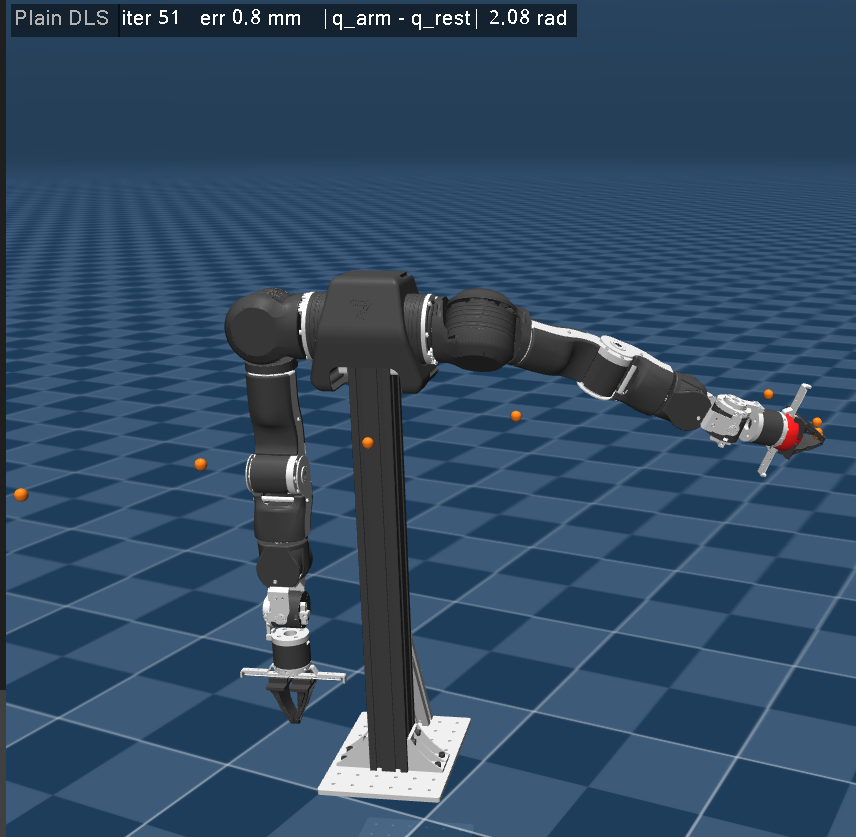
\includegraphics[height=7cm]{plain_dls.png}
        \caption{Plain DLS (per-joint damping only)}
    \end{subfigure}\hfill
    \begin{subfigure}[t]{0.48\textwidth}
        \centering
        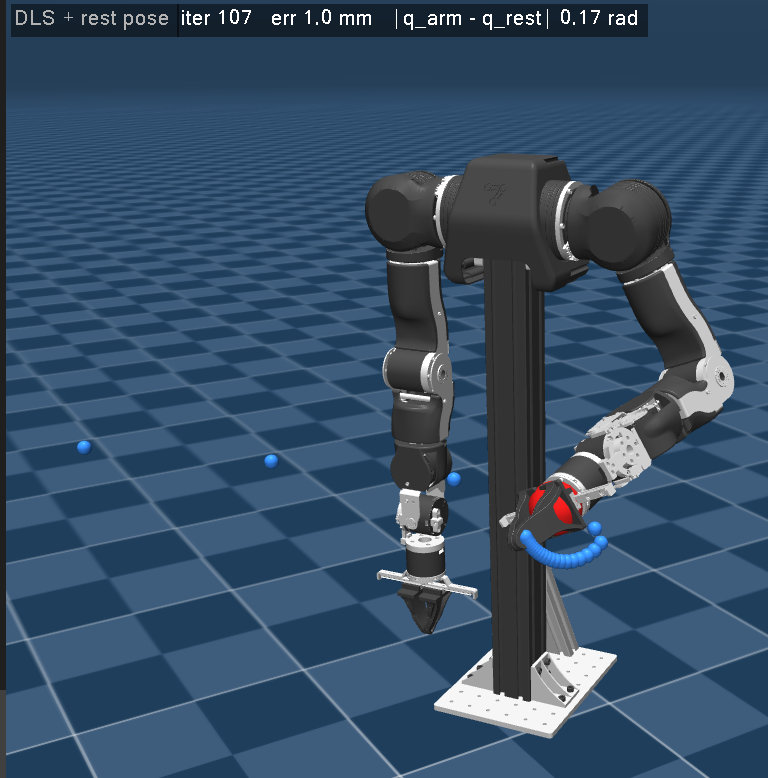
\includegraphics[height=7cm]{rest_dls.png}
        \caption{DLS with rest pull (and joint-limit damping)}
    \end{subfigure}
    \caption{\small{Comparison of plain DLS and DLS with the rest pull for the same target and initial state. With plain DLS the arm stretches straight toward the goal, whereas with the rest pull the arm stays near its resting configuration and the base takes up more of the motion.}}
    \label{fig:dls_comparison}
\end{figure}

Fig.~\ref{fig:dls_comparison} compares the two solvers. Plain DLS reaches
the target by moving the arm directly toward it, which drives the arm joints
far from their resting positions. With the rest pull, the arm keeps a posture
close to $\mathbf{q}^{\mathrm{rest}}$ and the base moves further to
compensate. Overall, the rest pull converges more slowly than plain DLS, but
it maintains a better arm posture throughout the motion.

\medskip
\noindent\textbf{Generalization.}
The damping and the rest pull share the same structure, a quadratic cost
$(\Delta\mathbf{q}+\mathbf{a})^{T}\mathbf{A}(\Delta\mathbf{q}+\mathbf{a})$
with a positive semi-definite weight $\mathbf{A}$ and a reference offset
$\mathbf{a}$. The damping term is the case $\mathbf{A}=\boldsymbol{\Lambda}\mathbf{W}$,
$\mathbf{a}=\mathbf{0}$, and the rest pull is the case $\mathbf{A}=\mathbf{R}$,
$\mathbf{a}=\boldsymbol{\delta}$. Theoretically, this allows any number of
secondary objectives to be added to the solver in the same way:
\begin{equation}
    \min_{\Delta\mathbf{q}}
    \left\{
        \|\mathbf{e}-\mathbf{J}\Delta\mathbf{q}\|^2
        + \sum_{k}
        \left(\Delta\mathbf{q}+\mathbf{a}_k\right)^{T}\mathbf{A}_k
        \left(\Delta\mathbf{q}+\mathbf{a}_k\right)
    \right\}
    \;\Rightarrow\;
    \left(\mathbf{J}^{T}\mathbf{J}+\sum_{k}\mathbf{A}_k\right)\Delta\mathbf{q}
    = \mathbf{J}^{T}\mathbf{e}-\sum_{k}\mathbf{A}_k\mathbf{a}_k
    \label{eq:general_objective}
\end{equation}
Each new objective only adds a weight to the left-hand matrix and a force
term to the right-hand side, so the linear solve keeps the same form and
the same cost. For the single-arm solver considered here, this
formulation worked well. However, it does not extend cleanly to the
two-arm case treated in the next subsection. All of the weighted terms
compete with the task term through the same matrix, so each added
objective slows convergence, and the soft rest pull shifts the
equilibrium away from zero error. However, with two arms sharing one base, this trade-off becomes severe enough that the soft-weight formulation no
longer works well, which motivates a different treatment of the
secondary objective.


\newpage
% TODO next: extension to two arms (shared base).

\subsection*{Bimanual Arm Integration}
The single-arm solver was extended to the full robot, with the mobile base
shared by both arms. The configuration now has $n=18$ degrees of freedom: the
four base joints, the seven left-arm joints and the seven right-arm joints. The joint-state $\mathbf{q}$ is now defined as:
\begin{equation}
    \mathbf{q} = [\ \mathbf{q}_B;\ \mathbf{q}_L;\ \mathbf{q}_R]= [\ x,\ y,\ lift,\ \psi, \ q_{L_1},\ ...,\ q_{L_7}\,\ q_{R_1}, ...,\ q_{R_7}]^T \in\mathbb{R}^{18}
\end{equation}

Each hand has its own position target, $\mathbf{p}^{L}_{\mathrm{target}}$ for the
left hand and $\mathbf{p}^{R}_{\mathrm{target}}$ for the right hand, and each hand
has its own Jacobian and error vector. With the newly defined $\mathbf{q}$ the two Jacobians share
the base columns and act on only their own arm:
\begin{equation}
    \mathbf{J}_L = \begin{bmatrix}\mathbf{B}_L & \mathbf{A}_L & \mathbf{0}\end{bmatrix},
    \qquad
    \mathbf{J}_R = \begin{bmatrix}\mathbf{B}_R & \mathbf{0} & \mathbf{A}_R\end{bmatrix}
    \label{eq:bimanual_jacobians}
\end{equation}
where $\mathbf{B}_L$ and $\mathbf{B}_R$ are the columns for the base joints and
$\mathbf{A}_L$ and $\mathbf{A}_R$ the columns for the arm joints. The right target
was generated at a random distance of up to $0.5$ m from the left target, in a
random direction.

\paragraph*{Averaged-step integration.}
The first integration reused the single-arm solver directly. Each arm was
solved independently with \eqref{eq:rest_normal}, using the base and its own
arm, which gives a step $(\Delta\mathbf{q}_b^{L},\Delta\mathbf{q}_L)$ for the left
hand and $(\Delta\mathbf{q}_b^{R},\Delta\mathbf{q}_R)$ for the right hand. Since both
solutions move the same base, the base step was averaged,
\begin{equation}
    \Delta\mathbf{q}_b = \tfrac{1}{2}\left(\Delta\mathbf{q}_b^{L}+\Delta\mathbf{q}_b^{R}\right)
\end{equation}
while each arm kept its own step, and the new state was used to recompute both
errors at the next iteration.


\paragraph*{Convergence issue.}
Compared with the single-arm case, the averaged-step integration converged
much more slowly and, for most target pairs, stopped with a residual error
(Table~\ref{tab:bimanual_showcase}).

First, the averaged step is not the step that either solve assumed. Each arm
computed its own step assuming that the full base step $\Delta\mathbf{q}_b^{L}$
(or $\Delta\mathbf{q}_b^{R}$) would be taken, and chose its arm joints to
compensate. After averaging, the base moves differently, so neither hand
follows its predicted motion. When the two targets require opposite base
motions, the two base steps partly cancel, and the combined step makes
slow progress toward either target.

Second, the rest pull changes the equilibrium of the shared base. Stacking the
two tasks, convergence requires $\mathbf{J}^{T}\mathbf{e}=\mathbf{R}\boldsymbol{\delta}$
(Section on rest pull), and since the base joints have no resting position
($r_i=0$), the rows for the base joints reduce to
\begin{equation}
    \mathbf{B}_L^{T}\mathbf{e}_L + \mathbf{B}_R^{T}\mathbf{e}_R = \mathbf{0}
\end{equation}
This can be satisfied without $\mathbf{e}_L=\mathbf{e}_R=\mathbf{0}$ when the targets
require opposite base motions: the base is pulled equally by the two hands in
opposite directions, so it stops. The arm joints then balance the rest force
with a small residual error on each hand. In the showcase run, the two base
terms had a magnitude of $0.017$ each and summed to zero, while both hands
were still $16.7$~mm from their targets. A larger rest weight leaves a larger
residual (Table~\ref{tab:bimanual_sweep}).

\begin{table}[htbp]
    \centering
    \small
    \setlength{\tabcolsep}{5pt}
    \begin{tabular}{l c l c c}
        \hline
        Method & Iterations & Outcome &
        \shortstack{Final error\\L / R (mm)} &
        \shortstack{Distance from\\rest (rad)} \\
        \hline
        1. Single arm (left + base) & 35 & reached & 1.0 & 0.17 \\
        2. Averaged base step & 265 & stalled & 53.4 / 53.4 & 1.42 \\
        3. Stacked, same weight & 205 & stalled & 16.7 / 16.7 & 1.60 \\
        4. Stacked, weight $2\times10^{-5}$ & 40 & reached & 0.9 / 0.8 & 2.36 \\
        \hline
    \end{tabular}
    \caption{\small{Showcase target pair. The left target is in front of the robot and the right target is behind it on the right, so the base must move forward for one hand and backward for the other. Both targets are reachable together: the stacked solve without a rest weight reaches them in 40 iterations.}}
    \label{tab:bimanual_showcase}
\end{table}

\paragraph*{Results.}
Table~\ref{tab:bimanual_benchmark} repeats the comparison over 40 random target
pairs. The averaged-step solver reached the tolerance in only 1 of 40
runs, and the stacked solver with the same rest weight in none. Stacking alone
does not fix the problem, since the rest weight is still the cause of the
stall. With a tiny rest weight, the stacked solver reached 37 of 40 targets with
a median of 30 iterations; the 3 failures are target pairs that no setting can
reach. The \textcolor{blue}{\href{https://youtu.be/Ey7bL1Zsx1M}{comparison video}} shows the simulation of the
showcase pair for these methods.

\begin{table}[htbp]
    \centering
    \small
    \setlength{\tabcolsep}{5pt}
    \begin{tabular}{l c c c c}
        \hline
        Method & Reached &
        \shortstack{Median\\iterations} &
        \shortstack{Final error (mm)\\median / max} &
        \shortstack{Distance from\\rest, median (rad)} \\
        \hline
        1. Single arm & 40/40 & 30 & 1.0 / 1.0 & 0.17 \\
        2. Averaged & 1/40 & 292 & 36.2 / 229.7 & 1.09 \\
        3. Stacked, same weight & 0/40 & 212 & 10.1 / 212.4 & 1.18 \\
        4. Stacked, tiny weight & 37/40 & 30 & 0.9 / 210.1 & 1.77 \\
        \hline
    \end{tabular}
    \caption{\small{Benchmark over 40 random target pairs.}}
    \label{tab:bimanual_benchmark}
\end{table}

\begin{table}[htbp]
    \centering
    \begin{tabular}{l l c c}
        \hline
        Rest weight & Outcome & Final error (mm) & Distance from rest (rad) \\
        \hline
        none & reached & $<1$ & 2.36 \\
        $\le 10^{-4}$ & reached & $<1$ & 2.33--2.36 \\
        $5\times10^{-4}$ & stalled & 2.4 & 1.69 \\
        $4\times10^{-3}$ & stalled & 16.7 & 1.60 \\
        $10^{-2}$ & stalled & 36.9 & 1.49 \\
        \hline
    \end{tabular}
    \caption{\small{Effect of the rest weight on the stacked solver (showcase targets).}}
    \label{tab:bimanual_sweep}
\end{table}

The sweep shows the trade-off directly. A weight small enough to reach both
targets ($\le10^{-4}$) leaves the arms as far from rest as with no rest weight
(2.33--2.36~rad), so the rest pull has effectively disappeared, whereas a weight
large enough to hold posture stalls with a residual error that grows with the
weight. The soft rest weight cannot provide both accuracy and posture for two
arms.


\paragraph*{Toward a resolution.}
The results above show two separate failures, and they have different causes.

\emph{Why independent solves disagree.}
Each hand moves according to its own Jacobian, so for a step $\Delta\mathbf{q}$ the first-order hand displacements are
\begin{equation}
    \Delta\mathbf{x}_L = \mathbf{B}_L\Delta\mathbf{q}_b + \mathbf{A}_L\Delta\mathbf{q}_L,
    \qquad
    \Delta\mathbf{x}_R = \mathbf{B}_R\Delta\mathbf{q}_b + \mathbf{A}_R\Delta\mathbf{q}_R
\end{equation}
The base columns $\mathbf{B}_L$ and $\mathbf{B}_R$ appear in both equations, so the two hands are coupled through the base. Solving each arm separately ignores this: the left solve plans the displacement $\mathbf{B}_L\Delta\mathbf{q}_b^{L}+\mathbf{A}_L\Delta\mathbf{q}_L$ as if only the left hand existed, and the right solve does the same. When the averaged base step $\tfrac12(\Delta\mathbf{q}_b^{L}+\Delta\mathbf{q}_b^{R})$ is applied instead, the left hand actually moves by
\begin{equation}
    \Delta\mathbf{x}_L^{\mathrm{actual}}
    = \Delta\mathbf{x}_L^{\mathrm{planned}}
    + \tfrac12\mathbf{B}_L\left(\Delta\mathbf{q}_b^{R}-\Delta\mathbf{q}_b^{L}\right)
\end{equation}
and symmetrically for the right hand. The prediction error is zero only when the two base steps agree. In the showcase, one target needs the base to move forward and the other needs it to move backward, so the two steps are opposite and the prediction error is at its largest. The arms compensate for a base motion that never happens, and both hands fall short.

\emph{Why a stacked solve does not have this problem.}
The coupling is exactly what the stacked Jacobian describes. Writing both tasks in one system, as is done for multiple end effectors in~\cite{bussKim2004},
\begin{equation}
    \underbrace{\begin{bmatrix}\mathbf{e}_L\\ \mathbf{e}_R\end{bmatrix}}_{\mathbf{e}}
    \approx
    \underbrace{\begin{bmatrix}\mathbf{B}_L & \mathbf{A}_L & \mathbf{0}\\ \mathbf{B}_R & \mathbf{0} & \mathbf{A}_R\end{bmatrix}}_{\mathbf{J}\,\in\,\mathbb{R}^{6\times 18}}
    \Delta\mathbf{q}
\end{equation}
and solving it once with the damped step used for a single arm,
\begin{equation}
    \Delta\mathbf{q}_{\mathrm{task}}=\mathbf{J}^{\#}\mathbf{e},
    \qquad
    \mathbf{J}^{\#}=\left(\mathbf{J}^{T}\mathbf{J}+\boldsymbol{\Lambda}\mathbf{W}\right)^{-1}\mathbf{J}^{T}
    \label{eq:stacked_dls}
\end{equation}

\newpage
with the per-joint damping $\boldsymbol{\Lambda}$ and the joint-limit weights $\mathbf{W}$ unchanged, gives a single step that reduces both errors at the same time to first order, because the shared base columns appear in both rows. The base step is a compromise chosen for both hands together, and the arm joints, whose columns belong to one hand only, absorb what the base cannot provide for each hand. Opposite base demands are therefore not a conflict. There are 18 joints for 6 task constraints, so the system has a 12-dimensional redundancy, which is enough to satisfy both targets exactly. This agrees with the showcase result, where the stacked solve without a rest weight reached both targets in 40 iterations (Table~\ref{tab:bimanual_showcase}). The next subsection builds on this form to construct a live full-body solver.


\subsection*{Stacked Full-Body IK with Orientation Control}
The stacked formulation above was extended into a live full-body IK solver for the base, the lift and both arms. Each hand now contributes six rows instead of three: the three position rows used so far plus three orientation rows~\cite{schinstock1994}, built from the angular part $\mathbf{J}_{\omega}$ of its Jacobian and the orientation error $\mathbf{e}_{\omega}$ between the target and current hand orientation,
\begin{equation}
    \mathbf{J}_{k}=\begin{bmatrix}\mathbf{J}_{v,k}\\ \mathbf{J}_{\omega,k}\end{bmatrix},
    \qquad
    \mathbf{e}_{k}=\begin{bmatrix}\mathbf{e}_{p,k}\\ \mathbf{e}_{\omega,k}\end{bmatrix},
    \qquad k\in\{L,R\}
\end{equation}
so the full stacked system has up to $12$ rows and $18$ columns. The solver can switch which parts are active:
\begin{itemize}[nosep]
    \item the left hand, the right hand, or both;
    \item position only, or position with orientation, for each active hand;
    \item whether the base and the lift are free to move.
\end{itemize}
This is done by selecting rows and columns before the solve. With a row-selection matrix $\mathbf{S}_t$ that keeps the active task rows and a column-selection matrix $\mathbf{S}_q$ that keeps the enabled joints,
\begin{equation}
    \mathbf{J}_{\mathrm{sel}}=\mathbf{S}_t\mathbf{J}\mathbf{S}_q,
    \qquad
    \mathbf{e}_{\mathrm{sel}}=\mathbf{S}_t\mathbf{e},
    \qquad
    \Delta\mathbf{q}
    = \mathbf{S}_q\left(\mathbf{J}_{\mathrm{sel}}^{T}\mathbf{J}_{\mathrm{sel}} + \boldsymbol{\Lambda}_{\mathrm{sel}}\mathbf{W}_{\mathrm{sel}}\right)^{-1}\mathbf{J}_{\mathrm{sel}}^{T}\mathbf{e}_{\mathrm{sel}}
    \label{eq:selected_dls}
\end{equation}
where $\boldsymbol{\Lambda}_{\mathrm{sel}}$ and $\mathbf{W}_{\mathrm{sel}}$ are the damping and weights of the enabled joints, and disabled joints receive zero update. The same linear solve therefore covers every mode, from one hand in position only up to both hands with full pose control. This solver has no secondary null-space term: the redundancy left by the task is resolved only by the damping.

\newpage
The solver runs live in the simulator, with a GUI to switch between these modes (Fig.~\ref{fig:live_gui}; \textcolor{blue}{\href{https://youtu.be/Kn5jznpRHcw}{demonstration video}}).

\begin{figure}[htbp]
    \centering
    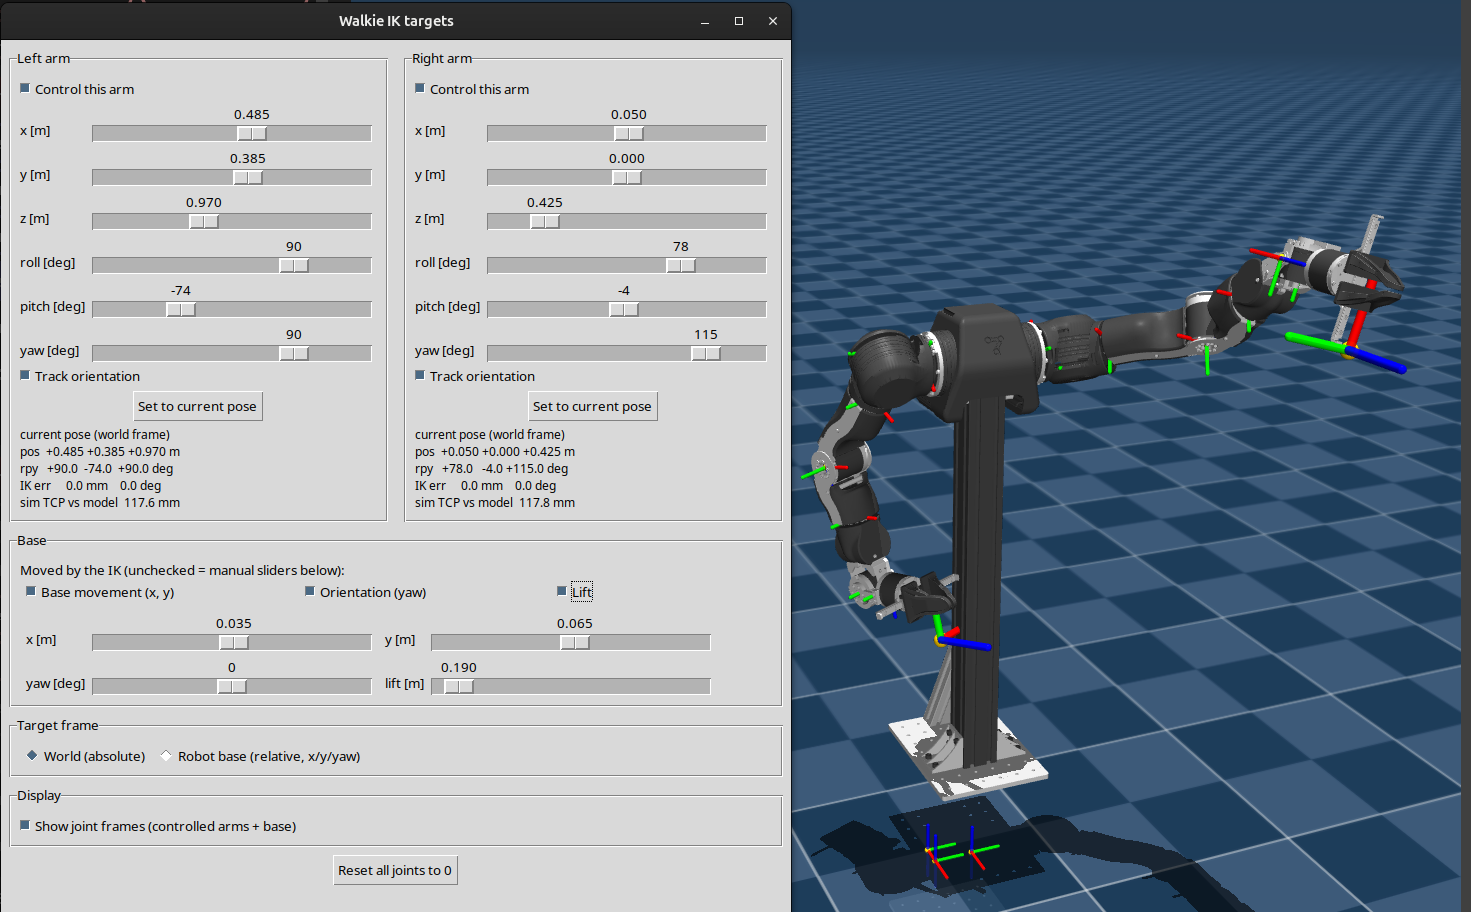
\includegraphics[width=0.9\linewidth]{live_ik_gui.png}
    \caption{\small{Live full-body IK interface, with controls for the active hands, orientation control, and base and lift enable.}}
    \label{fig:live_gui}
\end{figure}


The number of spare degrees of freedom depends on the mode (Table~\ref{tab:live_modes}). Each added task row or removed joint reduces the freedom that a secondary objective, such as a posture term, can use.

\begin{table}[htbp]
    \centering
    \small
    \setlength{\tabcolsep}{6pt}
    \begin{tabular}{l c c c}
        \hline
        Mode & Rows & Joints & Spare DOF \\
        \hline
        Both hands, position, base and lift on & 6 & 18 & 12 \\
        Both hands, position and orientation, base and lift on & 12 & 18 & 6 \\
        Both hands, position and orientation, base and lift off & 12 & 14 & 2 \\
        One hand, position and orientation, base and lift on & 6 & 11 & 5 \\
        One hand, position, base and lift off & 3 & 7 & 4 \\
        One hand, position and orientation, base and lift off & 6 & 7 & 1 \\
        \hline
    \end{tabular}
    \caption{\small{Task rows, enabled joints and spare degrees of freedom (joints minus rows) for several modes, assuming full-rank Jacobians.}}
    \label{tab:live_modes}
\end{table}

\newpage
\subsection*{Posture as a Null-Space Task}
\emph{Why the posture should not be a weight.}
The initial plan was to keep the posture as a soft weight, as in the single-arm solver. The sweep in Table~\ref{tab:bimanual_sweep} shows why this does not carry over: a weight small enough to reach both targets leaves the posture unchanged, and a weight large enough to hold the posture stalls the task. A soft weight trades task accuracy against posture through the same cost, and with two arms sharing a base the equilibrium of that trade is a point with non-zero error (the cancellation of the base terms discussed above). Scheduling the weight down as the error shrinks does not remove the problem either, since it only helps if the fade begins above the error at which the solver stalls.

The redundancy found above suggests a different use. In the position-only two-arm case there are 12 spare degrees of freedom (Table~\ref{tab:live_modes}), so there are many joint motions that change the hand positions by nothing, and the posture can be corrected using only those. This is the classical null-space approach~\cite{nakamura1987,schinstock1994}: the task has priority, and the posture acts only on what the task leaves free,
\begin{equation}
    \Delta\mathbf{q}
    = \mathbf{J}^{\#}\mathbf{e}
    + \left(\mathbf{I}-\mathbf{J}^{\#}\mathbf{J}\right)\mathbf{K}\left(\mathbf{q}^{\mathrm{rest}}-\mathbf{q}\right)
    \label{eq:stacked_nullspace}
\end{equation}
where $\mathbf{K}$ is a diagonal gain that is zero for joints without a resting position. The factor $(\mathbf{I}-\mathbf{J}^{\#}\mathbf{J})$ removes the part of the posture correction that would move the hands, since $\mathbf{J}(\mathbf{I}-\mathbf{J}^{\dagger}\mathbf{J})=\mathbf{0}$ for the exact pseudoinverse. In implementation the damped $\mathbf{J}^{\#}\mathbf{J}$ is replaced by a soft projector built from the singular value decomposition of $\mathbf{J}$, with a small damping on the singular values, so that near-singular directions are not treated as free. The choice of projector is known to distort the secondary motion, so the secondary task may not be executed in the best attainable way~\cite{lenarcic1998}; the posture reached in practice is therefore an approximation of the desired one. The posture term then changes the arm configuration without changing the hand positions, so it no longer competes with the task and no longer shifts the equilibrium away from zero error. This replaces the choice of a single weight with a priority between the task and the posture, which is why the weight sweep no longer applies. Adding orientation rows reduces the null space (Table~\ref{tab:live_modes}), so the posture term has less freedom in those modes.

We initially took this formulation to be new for our platform. It was in fact formalized by Nakamura et al.~\cite{nakamura1987} and refined by Lenar\v{c}i\v{c}~\cite{lenarcic1998} decades ago. This formulation follows the task-priority framework of Nakamura et al.~\cite{nakamura1987}, with the choice of projector discussed by Lenar\v{c}i\v{c}~\cite{lenarcic1998}. In this work it is applied to a mobile bimanual platform with a shared base, where the benchmarks above show that the weighted formulation stalls and the null-space formulation does not.

\paragraph{Results.}
Table~\ref{tab:nullspace_results} compares the three variants on the same 32 targets and benchmark as Table~\ref{tab:bimanual_sweep}. The weighted rest pose reaches none of the targets. It stalls at a median error of 9.49\,mm, which is the non-zero equilibrium described above. It stays closest to the rest pose (1.09\,rad), but only because the posture term is holding the arms back from the task. Removing the posture term entirely gives the opposite outcome. Every target is reached in a median of 25 iterations, but the arms drift 1.71\,rad from rest, since nothing constrains how the solver uses the 12 spare degrees of freedom.

Projecting the rest pose into the null space combines the two. Convergence is unchanged (31/32 reached, median 25 iterations, median final error 0.02\,mm), so the posture term does not slow the task. Distance from rest drops to 1.20\,rad, which recovers most of the posture lost in the unconstrained case and comes within 0.11\,rad of the weighted solver, which never reaches its targets. The one target not reached ends at 1.9\,mm.
% TODO: one-line cause for the 1.9 mm case, e.g. a near-singular target where the
% damped soft projector lets a small part of the posture correction leak into the task directions.

Figure~\ref{fig:rest_vs_norest} shows the final configuration for the same target with and without the null-space posture term. The hand positions are identical, but without the posture term the arms settle into [describe, e.g. raised elbows / twisted wrists], while with it they stay close to the resting configuration. A side-by-side video of all three solvers on the benchmark is provided \textcolor{blue}{\href{https://youtu.be/3rgqf_vf3_w}{here}}.

\begin{table}[htbp]
    \centering
    \small
    \setlength{\tabcolsep}{5pt}
    \begin{tabular}{l c c c c}
        \hline
        Method & Reached &
        \shortstack{Median iter.\\to 1~mm} &
        \shortstack{Final error (mm)\\median / max} &
        \shortstack{Distance from\\rest, median (rad)} \\
        \hline
        Weighted rest pose & 0/32 & -- & 9.49 / 27.9 & 1.09 \\
        Null space, no rest pose & 32/32 & 25 & 0.00 / 0.8 & 1.71 \\
        Null-space rest pose & 31/32 & 25 & 0.02 / 1.9 & 1.20 \\
        \hline
    \end{tabular}
    \caption{\small{Two-arm position-only IK on 32 targets. Distance from rest is the norm of $\mathbf{q}-\mathbf{q}^{\mathrm{rest}}$ over joints with a resting position.}}
    \label{tab:nullspace_results}
\end{table}

\begin{figure}[htbp]
    \centering
    \begin{subfigure}[t]{0.48\textwidth}
        \centering
        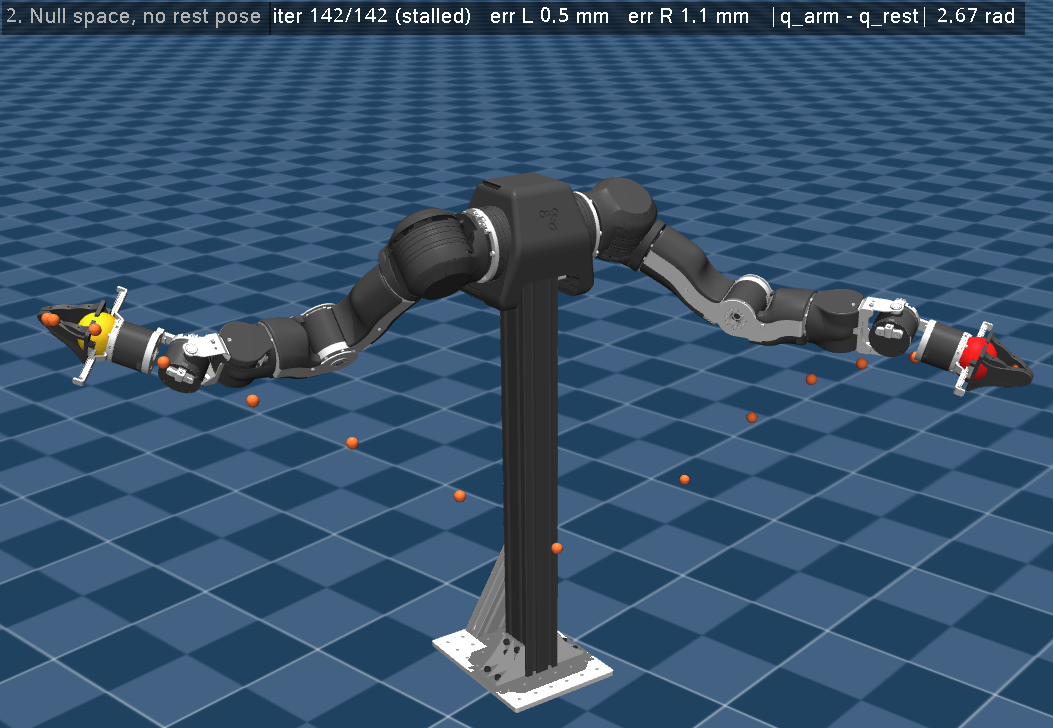
\includegraphics[height=5cm]{nullplain.png}
        \caption{Null space, no rest pose}
        \label{fig:final_no_rest}
    \end{subfigure}\hfill
    \begin{subfigure}[t]{0.48\textwidth}
        \centering
        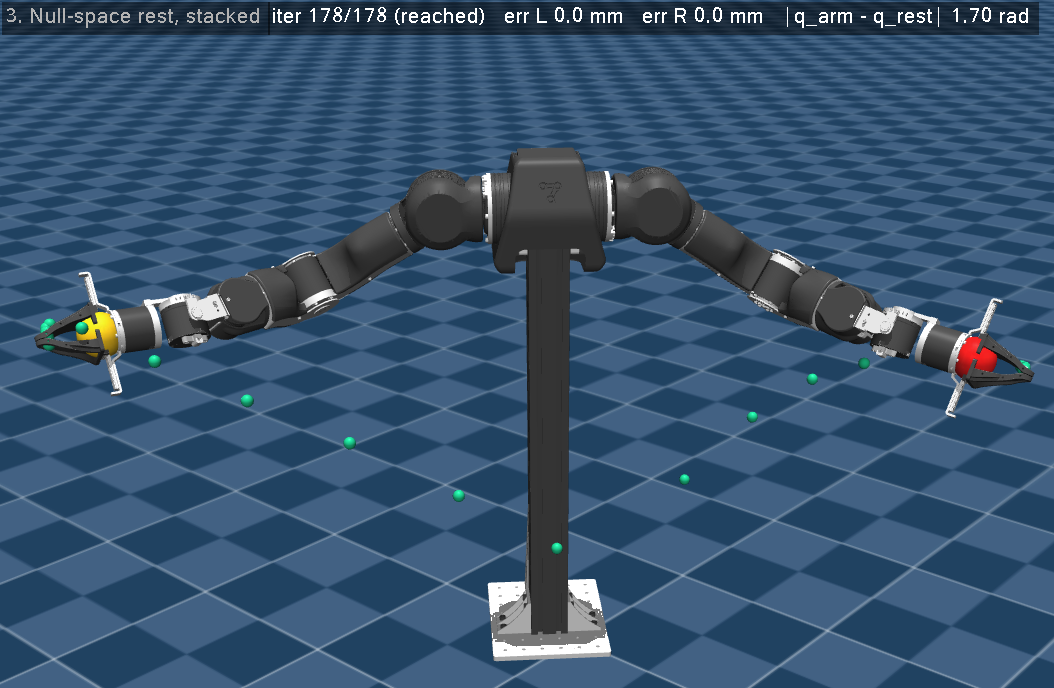
\includegraphics[height=5cm]{nullrest.png}
        \caption{Null-space rest pose}
        \label{fig:final_nullspace_rest}
    \end{subfigure}
    \caption{\small{Final configuration for the same target. Both reach the target. The posture term in (b) keeps the arms near the resting configuration using only joint motions that do not move the hands.}}
    \label{fig:rest_vs_norest}
\end{figure}
\newpage
\subsection*{Summary and Next Steps}
This section developed the inverse kinematics solver from the Jacobian pseudoinverse to damped least squares~\cite{buss2009}, then to per-joint damping, joint-limit damping and a rest-position pull for a single arm. Extending it to two arms showed that a soft rest weight cannot provide both accuracy and posture when the arms share a base. A stacked solve of both hands, with the posture applied in the null space of the task~\cite{nakamura1987}, resolved this, and the same stacked solve with row and column selection forms the live full-body solver with position and orientation control.

The current solver is a local, differential method. It computes one joint-state update toward the current targets and does not plan a path, avoid obstacles or choose where the base should go. Two directions follow from this. The first is obstacle avoidance. Maciejewski and Klein~\cite{maciejewski1985} use the redundancy of a manipulator for this purpose: at each step the point on the manipulator closest to an obstacle is identified, and a velocity away from the obstacle surface is assigned to it as a secondary goal, resolved in the null space of the primary end-effector task. This has the same structure as the posture term used here, with the rest-pose pull replaced by an obstacle-avoidance velocity, so we plan to build avoidance for the arms and the mobile base on this approach. The same null space can also be used for the motion of the base, so that the redundancy left by the hands moves the base while the hands keep their targets. As Table~\ref{tab:live_modes} shows, this freedom shrinks when orientation is controlled, so how much the base can be driven this way in each mode will need to be evaluated.

The second direction is path planning and navigation for full-body control, which would produce a sequence of base poses and hand targets for the IK solver to track. This is expected to be a separate layer built on top of the IK solver, with the IK solver kept as the low-level tracking step, and it is planned together with the obstacle avoidance above so that the two share the same obstacle information.


\clearpage
% ============================================================
% SOFTWARE AND AGENT DEVELOPMENT -- added 22 October 2026
% Sources: walkie-ros/docs/migrations/01-pixi.md and 02-mujoco/;
% walkie-agent-v2/README.md; walkie-agent-ros/docs/architecture/
% agent.md, self-evolving-agent.md, manipulation.md; current source
% and pixi.toml files. Results summarize recorded development evidence.
% ============================================================

\providecommand{\migrationplaceholder}[2]{%
  \fbox{\begin{minipage}[c][#1][c]{0.88\linewidth}
    \centering\small\textit{#2}
  \end{minipage}}%
}

\section*{Software Infrastructure and Simulation Development}

\subsection*{Objectives and Relation to Whole-Body Control}

Alongside the inverse kinematics development, the robot software was
reorganized to provide a reproducible environment for integrating and
testing the Walkie platform. This work focused on two changes in
\textcolor{blue}{\href{https://github.com/EIC-Robocup-2026/walkie-ros}{\texttt{walkie-ros}}}: moving the development environment from a system-wide
ROS~2 installation to Pixi, and introducing a MuJoCo simulation of the
complete robot alongside the existing Gazebo setup.

The earlier OpenArm-based experiments provide an environment for studying
the coordinated base--arm solver. The full Walkie simulation extends the
infrastructure to include the robot description, controllers, sensor
interfaces, and navigation stack. This establishes a platform for
subsequent integration of the solver with ROS~2. The migration itself
does not establish that the full-body IK solver has already been connected
to the complete robot or validated in a grasping task.

\subsection*{Migration from System ROS~2 to Pixi}

Previously, ROS~2 Jazzy was installed system-wide through the Ubuntu
package manager, with additional dependencies installed through
\texttt{rosdep}. Developers built a conventional ROS workspace and
manually sourced the ROS installation and workspace overlay. The new
workflow installs ROS~2 and its dependencies inside a project-local
Pixi environment, using the RoboStack Jazzy and conda-forge channels.

The dependency specification is stored in \texttt{pixi.toml}, while
\texttt{pixi.lock} records the resolved package versions. This makes the
software environment explicit and recreatable for the supported
Linux x86\_64 platform. ROS~2 remains the robot middleware, and
\texttt{colcon} remains the package build tool; Pixi manages the
environment and the commands used to build and run them.

\begin{table}[htbp]
    \centering
    \small
    \renewcommand{\arraystretch}{1.15}
    \begin{tabular}{p{0.18\linewidth} p{0.33\linewidth} p{0.36\linewidth}}
        \hline
        Aspect & Previous workflow & Updated workflow \\
        \hline
        ROS installation & System packages under \texttt{/opt/ros/jazzy}
            & Project-local environment managed by Pixi \\
        Dependencies & System packages installed with \texttt{rosdep}
            & Declared dependencies and a version lockfile \\
        Workspace & Repository inside a separate ROS workspace
            & Repository root used as the workspace \\
        Build and activation & Direct \texttt{colcon} invocation and manual sourcing
            & Pixi tasks invoke the build and activate the environment \\
        \hline
    \end{tabular}
    \caption{\small{Changes to the development workflow in \texttt{walkie-ros}.}}
    \label{tab:migration_pixi_workflow}
\end{table}

\newpage
The migration required compatibility work beyond adding an environment
file. The dependency list was reconciled with the ROS package manifests,
the compiler was pinned to GCC~13, and CMake was restricted to a version
compatible with the existing lidar SDK. Navigation dependencies were
updated to locate OpenVDB in the environment and build against the
available Boost version. Packages unavailable through the selected
channels are imported from source. A later update aligned the ROS
packages with a compatible RoboStack build set so that the required
MuJoCo control plugin could be installed.

The resulting workflow provides commands such as \texttt{pixi run build}
and \texttt{pixi run test}, together with automatic workspace activation.
Zenoh is selected consistently as the ROS~2 middleware in the Pixi
environment. The core workspace can therefore be built without a
system-wide ROS installation. Some hardware-specific dependencies,
including the proprietary camera SDK and CUDA requirements, still need
separate host setup; the migration does not yet cover every legacy
deployment path.

\subsection*{Gazebo-to-MuJoCo Simulation Migration}

The simulation work introduced a MuJoCo representation generated from the
existing Walkie Xacro/URDF description. A Python generator expands the
description and uses MuJoCo's \texttt{MjSpec} interface to construct the
MJCF model. It then adds simulator-specific elements, including the
floating base, actuators, collision settings, sensors, and an initial
configuration. Keeping the robot description as the common source
reduces the risk of maintaining inconsistent robot models.

A major modeling issue was the omnidirectional wheel contact. Each wheel
uses a thin capsule against an analytic floor plane, with an explicit
wheel--floor contact pair and direction-dependent friction. The
directional friction approximates the rolling and lateral-sliding
behavior of an omni wheel. Wheel velocity actuators drive a free
floating base through contact forces, allowing the base response to be
tested without directly prescribing its position. The migration also
identified a controller geometry mismatch: the distance from the base
center to a wheel was corrected from 0.252~m to 0.185~m.

The model is connected to ROS~2 through \texttt{mujoco\_ros2\_control}.
Dedicated launch files start the simulator, controller manager,
controllers, sensor publishers, and RViz; a second launch adds Nav2.
The sensor interfaces include an IMU, cameras, front and rear laser
scans, and a head-mounted 3D lidar. The two planar scans are merged into
the scan topic used by navigation. A separate MuJoCo controller
configuration allows the existing Gazebo configuration to remain
available during the transition.

\begin{figure}[htbp]
    \centering
    % Replace the box with:
    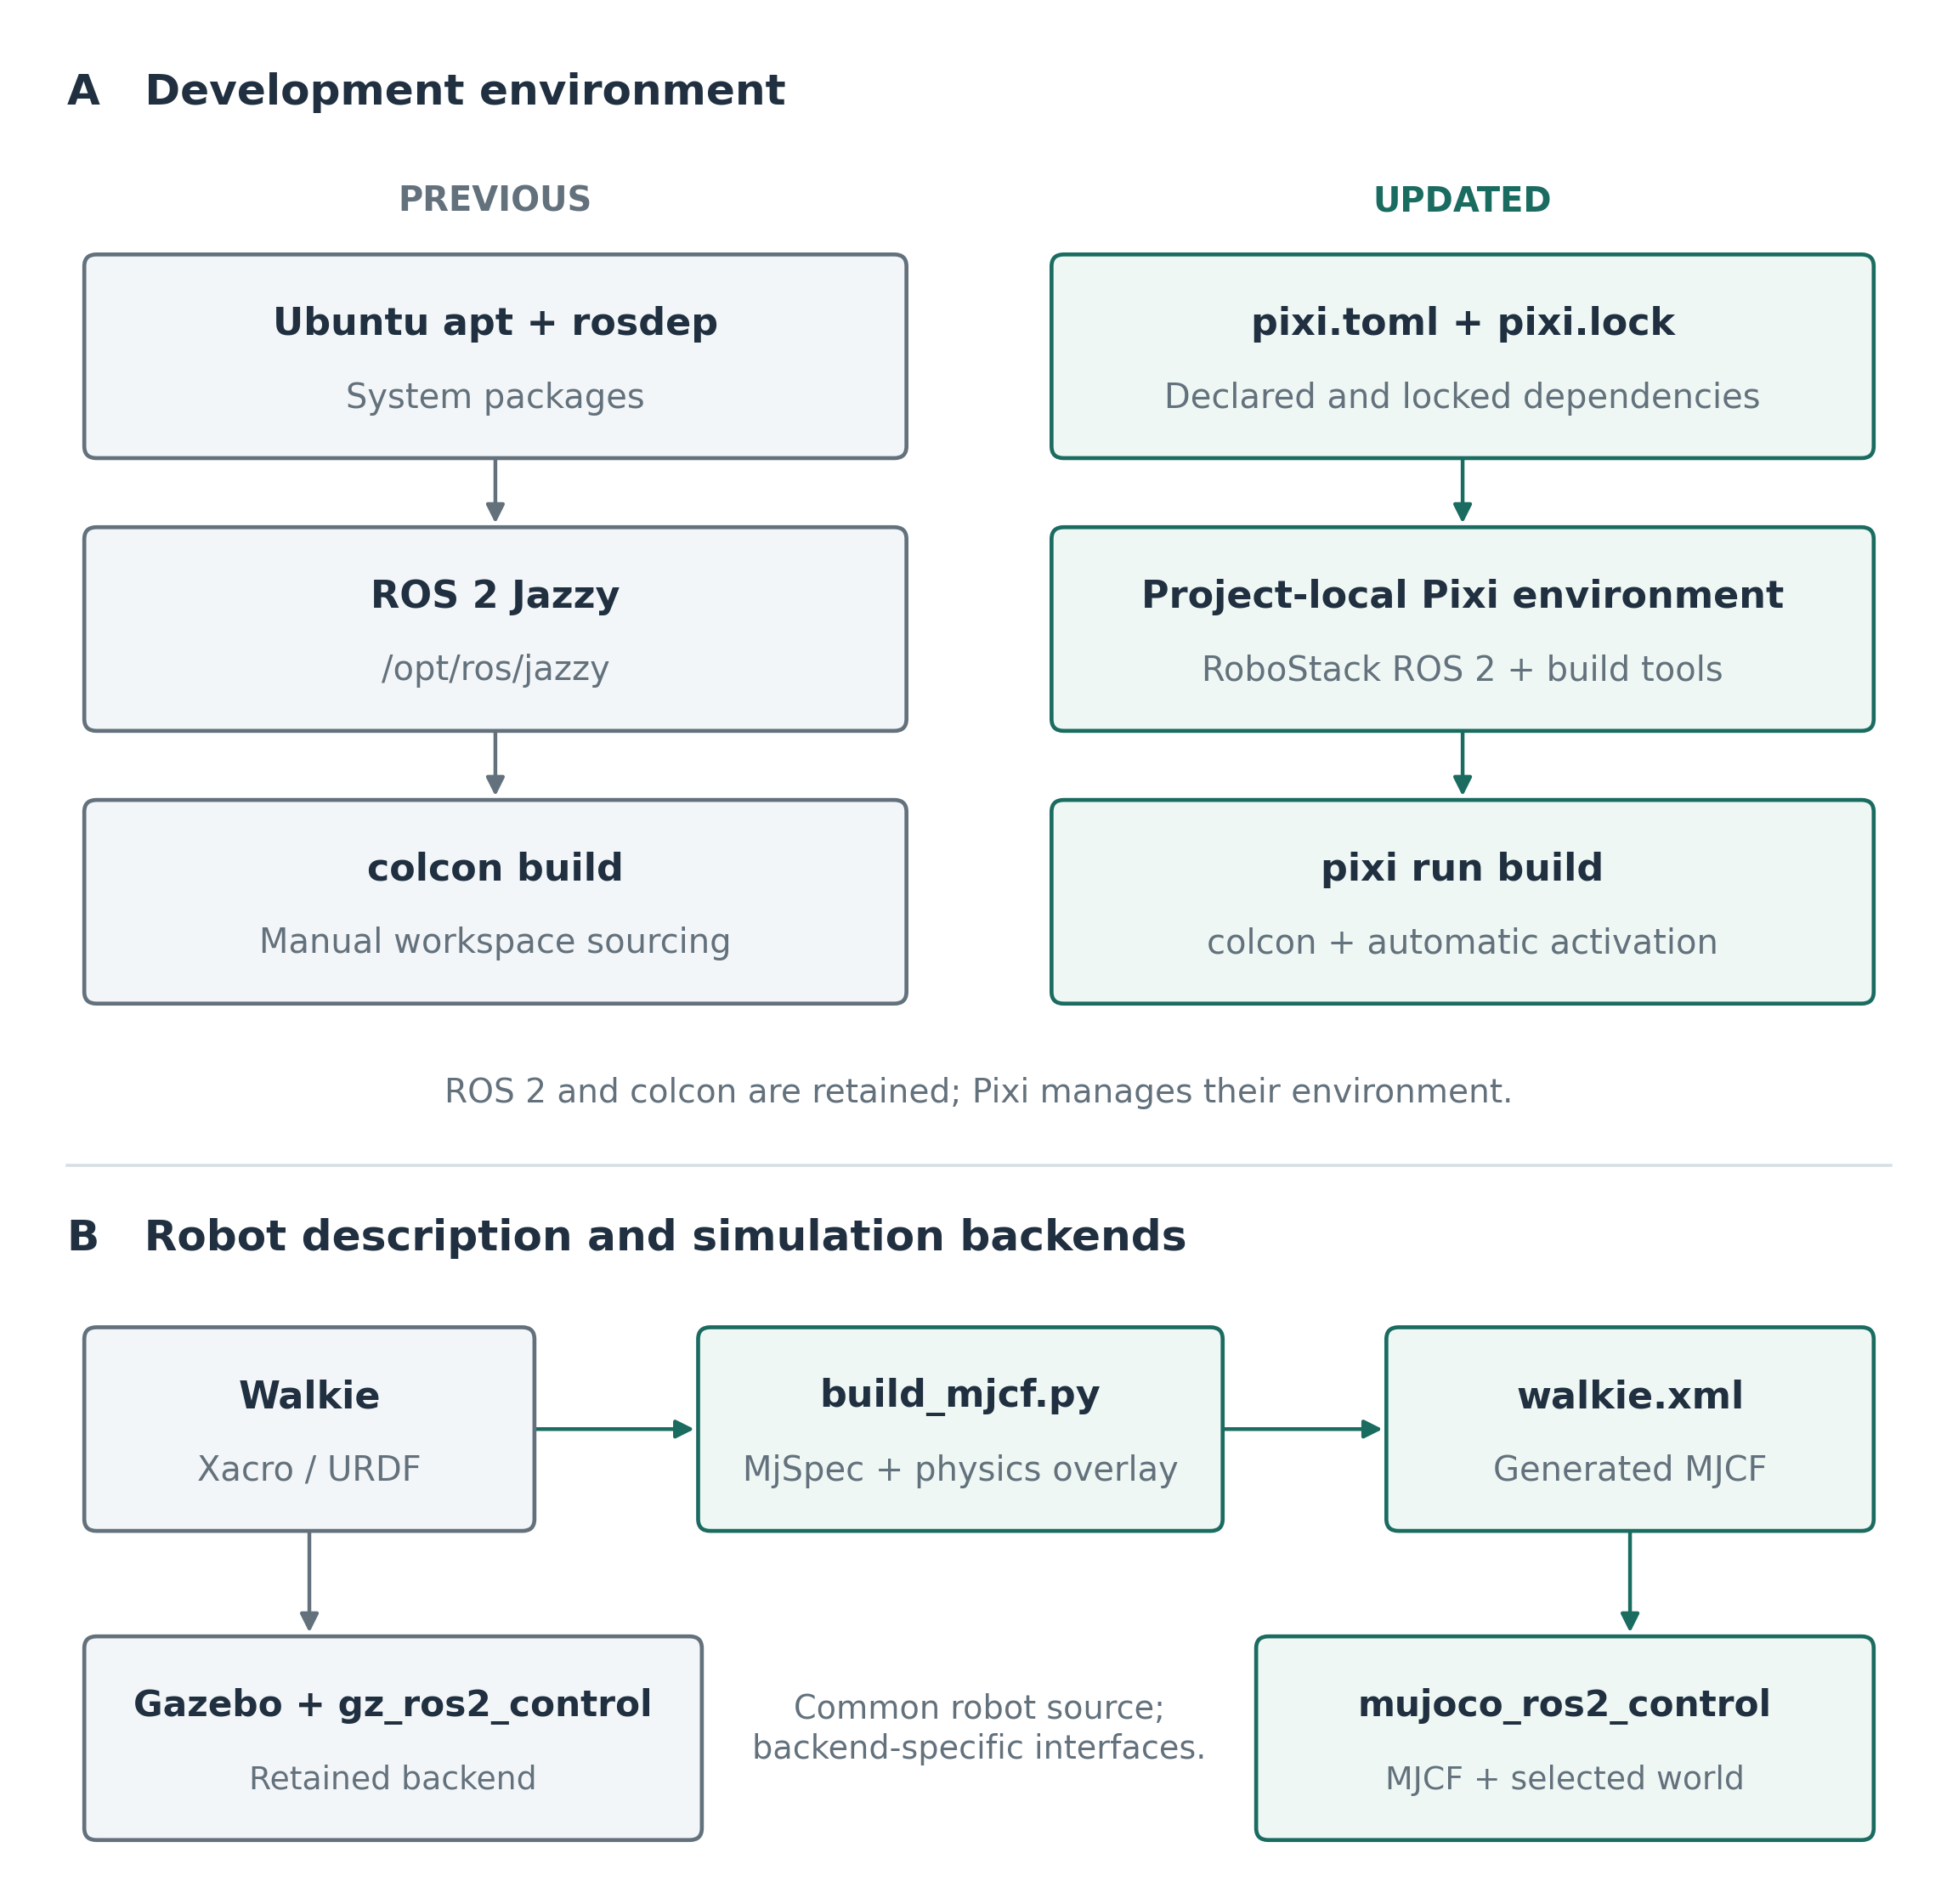
\includegraphics[width=0.90\linewidth]{migration_gazebo_mujoco_comparison.png}
    % \migrationplaceholder{4.3cm}{Insert a side-by-side image of Walkie in Gazebo and MuJoCo.\\
    % Use comparable viewpoints and label the two simulators.}
    \caption{\small{Comparison of the previous Gazebo setup and the
    MuJoCo model generated from the Walkie robot description.
    The images illustrate the model migration; they do not constitute
    a simulator accuracy benchmark.}}
    \label{fig:migration_gazebo_mujoco}
\end{figure}

\newpage
\subsection*{Environment Reconstruction and Reusable Worlds}

To extend testing beyond an empty floor, a reconstructed Chulapat 14
living room and kitchen were added as a named MuJoCo world. The
\texttt{walkie\_mujoco\_worlds} package contains the scene assets,
occupancy map, and a manifest specifying the available variants and
spawn poses. A launch can select the world by name and combine it with
the robot model. This separates environment assets from the robot
description and allows further test environments to be added using
the same format.

Two variants are available: a low-poly scene for general simulation and
a scene with baked lighting for visual inspection and camera work.
An integration issue arose when scene-wide export settings changed
the robot's inertia during model merging. The loader was updated so
that the robot retains ownership of the relevant model-wide physics
settings, and tests check that loading a world preserves the robot's
physical parameters.

\begin{figure}[htbp]
    \centering
    % Copied from walkie-ros/docs/assets/chula-pat14-6/.
    % Upload figures/migration_walkie_mujoco_room.png with this report.
    \IfFileExists{figures/migration_walkie_mujoco_room.png}{%
        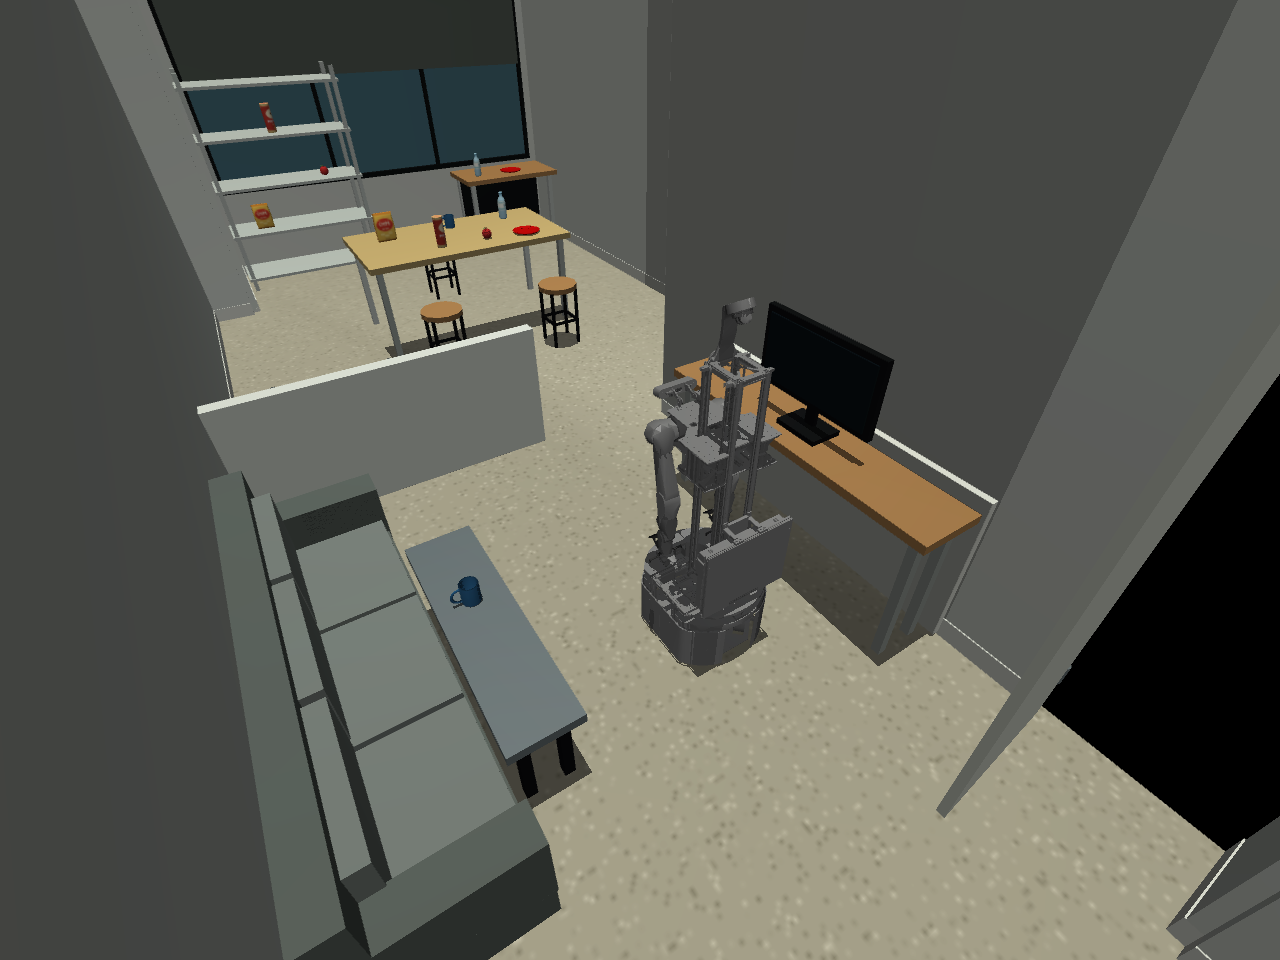
\includegraphics[width=0.87\linewidth]{migration_walkie_mujoco_room.png}%
    }{%
        \migrationplaceholder{5.5cm}{Insert migration\_walkie\_mujoco\_room.png:
        Walkie in the reconstructed Chula Pat14 room.}%
    }
    \caption{\small{Walkie placed in the reconstructed Chulapat 14
    living room, facing the kitchen. This existing project image
    illustrates scene integration; live AMCL localization and Nav2
    operation in this room remain to be verified.}}
    \label{fig:migration_mujoco_room}
\end{figure}

\newpage
\subsection*{Verification and Current Limitations}

Automated checks were added for the robot description, controller
interfaces, generated MJCF, and consistency between the URDF and
MoveIt semantic description. These include checks for missing links
and joints, incorrect controller interfaces, and a generated model
that no longer matches its source. Additional tests cover world
manifests, model merging, launch arguments, and installed world assets.

The recorded headless experiments activated the simulation controllers,
demonstrated base motion, and reached Nav2 goals on an empty floor.
A separate test world was used to demonstrate navigation around a
wall. These results establish a working ROS~2 simulation and navigation
path, but do not yet establish complete mobile manipulation.
MoveIt execution with MuJoCo and live navigation with AMCL in the
reconstructed room remain unverified. Some inertial and actuator
parameters are estimates, the wheel radius differs slightly between
the controller and contact model, and the current collision
configuration does not model base--furniture impacts. These limitations
must be considered when interpreting simulation results.

\begin{figure}[htbp]
    \centering
    % Replace with a screenshot from a documented navigation experiment:
    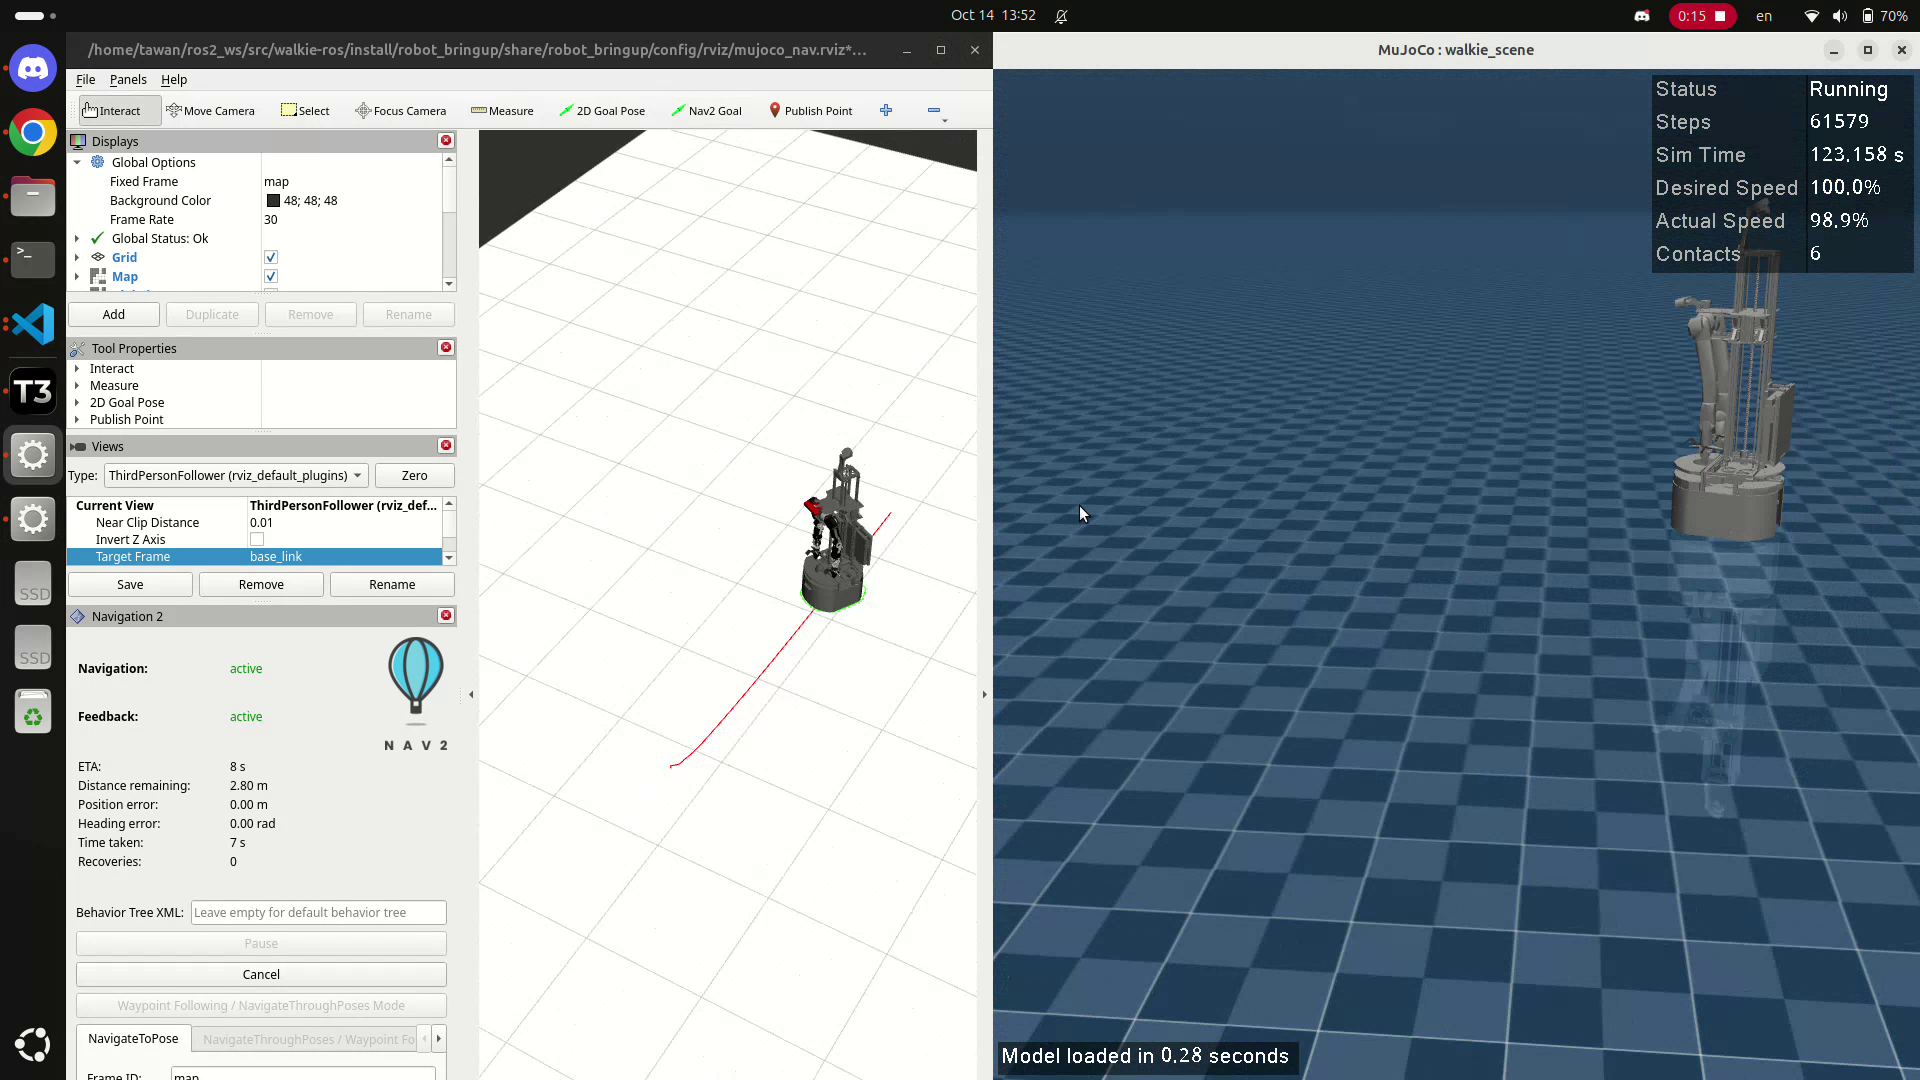
\includegraphics[width=0.90\linewidth]{migration_rviz_navigation.png}
    % \migrationplaceholder{4.3cm}{Insert an RViz navigation screenshot showing the map,
    % laser scan, planned path, robot pose, and goal.\\
    % Identify the test world and record the corresponding goal result.}
    \caption{\small{ROS~2 navigation visualization for the MuJoCo
    integration. A screenshot should be paired with the action result
    and test conditions when reporting successful navigation.}}
    \label{fig:migration_rviz_navigation}
\end{figure}

\clearpage
\section*{Agent Software Migration and Mahoraga Development Plan}

\subsection*{From \texttt{walkie-agent-v2} to \texttt{walkie-agent-ros}}

The agent software was restructured from \texttt{walkie-agent-v2}
into \texttt{walkie-agent-ros} to connect task-level reasoning more
directly to the ROS~2 robot stack. The earlier implementation was a
Python application managed with \texttt{uv}. It used LangChain and
LangGraph to coordinate a main agent with actuator, vision, and
database agents. Robot access was provided through
\texttt{walkie-sdk}, while a separate HTTP inference server
provided perception and speech services.

The new implementation is a ROS~2 Jazzy node built on RAI's
\texttt{ReActAgent}. Its tools communicate through ROS topics,
services, actions, and transforms. For example, navigation requests
are sent to Nav2 as action goals, and object-memory queries are sent
to \texttt{walkie-database} as service requests. This gives the agent
a direct interface to the existing robot software and a clearer
separation between task reasoning and robot execution.

This work establishes a smaller ROS-based foundation rather than
complete feature parity with the earlier multi-agent system.
The earlier perception workflows and competition-task implementations
have not all been ported. Robot control remains in
\texttt{walkie-ros}, object memory is accessed through
\texttt{walkie-database}, and the planned perception integration uses
\texttt{walkie-vision}.

\subsection*{Pixi Environment and Implemented Agent Functions}

The new agent repository also uses Pixi and RoboStack to manage
ROS~2, Python, build tools, and application dependencies. Its lockfile
records its own resolved environment, while using the same environment
management approach as \texttt{walkie-ros}. Source-built ROS message
packages and the Zenoh middleware have explicit build tasks; installing
the environment alone does not replace these steps.

Aligning the ROS communication stack required resolving a dependency
conflict between the OpenCV versions needed by RAI and a newer
RoboStack middleware build. The agent therefore builds the selected
Zenoh middleware from source. Simulation execution uses ROS simulation
time and the selected ROS domain so that the agent can communicate
with the running MuJoCo stack.

The current agent accepts text or speech-derived requests and uses a
fixed set of tools for speech, named-location navigation, bounded
relative movement, robot-pose lookup, and object-memory queries.
Named goals are resolved from configuration, and navigation tools
check the Nav2 action result, bound their waits, and request
cancellation on timeout. Speech output and operator-facing console
messages use separate topics. Optional robot-document retrieval
provides information about Walkie, while Langfuse tracing records
model calls and tool execution for inspection.

\begin{figure}[htbp]
    \centering
    % Copied from walkie-agent-ros/docs/assets/langfuse.png.
    % Upload figures/migration_agent_trace.png with this report.
    \IfFileExists{figures/migration_agent_trace.png}{%
        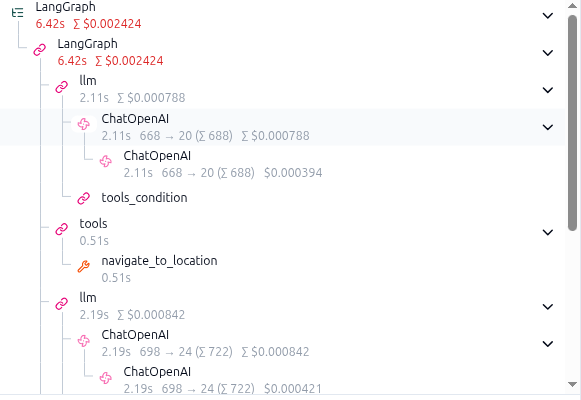
\includegraphics[height=8.0cm,keepaspectratio]{migration_agent_trace.png}%
    }{%
        \migrationplaceholder{6cm}{Insert migration\_agent\_trace.png:
        the Langfuse trace of agent and navigation-tool execution.}%
    }
    \caption{\small{An existing Langfuse trace of the ROS-based agent,
    showing model calls and navigation-tool execution. The displayed
    timings and costs describe this trace only and are not reported
    as a controlled performance benchmark.}}
    \label{fig:migration_agent_trace}
\end{figure}

Testing infrastructure includes a fake ROS robot and a scripted
language model. The test suite covers tool execution, navigation
failure reporting, human--robot interaction topics, and reset behavior
without requiring physical hardware or a paid model call. The
repository also provides a task for connecting the agent to the
MuJoCo simulation. These facilities support incremental integration;
real-robot agent deployment and agent-driven arm manipulation remain
future work.

\subsection*{Proposed Mahoraga Agent}

The next stage is the proposed self-evolving agent, named
\emph{Mahoraga} in the architecture documents. The current agent binds
a fixed tool set at startup. Mahoraga is intended to maintain an
explicit task plan, discover relevant tools, and compose reusable
operations while executing a task. In this design, self-evolving
refers to extending the available tool collection; it does not imply
online retraining of the language model. The architecture has been
documented, but this redesign has not yet been implemented.

The proposed development is organized around four capabilities:
\begin{enumerate}
    \item \textbf{Explicit planning and typed tools.}
    Maintain a task list with completion rules, and define small tools
    with typed inputs, outputs, and error conditions. Tools would be
    rebound at each reasoning step so that newly selected operations
    become available during a task.
    \\
    \item \textbf{Tool discovery and composition.}
    Search a larger tool catalogue using lexical and vector retrieval,
    then combine existing tools into validated sequences. A sequence
    would report which step failed and retain the evidence needed for
    recovery.

    \item \textbf{Controlled tool generation.}
    When existing tools cannot express a task, a dedicated component
    would propose a new implementation for execution in a sandbox.
    Access levels would constrain the robot and external interfaces
    available to generated code.

    \item \textbf{Simulation evaluation and review.}
    Evaluate generated operations in simulation, retain execution
    traces, and require human review before promoting successful tools
    into the maintained repository.
\end{enumerate}

Manipulation is planned to begin with mocked arm and skill interfaces
before connecting to robot-side execution. These mocks are also future
work; their eventual success would demonstrate task sequencing and
failure handling, not physical grasp success. The initial agent
manipulation scope excludes lift control. Connecting the full-body
solver, including its lift degree of freedom, will therefore require
a subsequent integration step.

\clearpage
\section*{Integration Status and Next Steps}

The migration establishes three complementary layers: a reproducible
software environment, a ROS-connected robot simulation, and an agent
that requests robot operations through defined interfaces. The IK
solver remains the motion-level component described earlier in this
report. The proposed integration is for the agent to select a task
and request a robot-side skill, while the motion-planning and control
layers determine and execute the base and arm motion.

\begin{table}[htbp]
    \centering
    \small
    \renewcommand{\arraystretch}{1.16}
    \begin{tabular}{p{0.20\linewidth} p{0.33\linewidth} p{0.34\linewidth}}
        \hline
        Component & Current evidence & Next validation step \\
        \hline
        Pixi environment &
        Manifests, lockfiles, and build tasks in both repositories &
        Reproduce installation and build on a second supported computer \\

        MuJoCo and Nav2 &
        Recorded controller activation and navigation tests; model checks &
        Verify live AMCL and navigation in the reconstructed room \\

        ROS-based agent &
        Implemented tools, fake-robot tests, and simulation launch task &
        Record repeatable language-to-navigation trials and failure cases \\

        Whole-body manipulation &
        IK experiments reported above; ROS integration remains to be completed &
        Connect the solver to robot-side execution and measure tracking errors \\

        Mahoraga &
        Architecture and phased implementation plan &
        Implement typed tools, task tracking, and validated composition first \\
        \hline
    \end{tabular}
    \caption{\small{Current integration status and proposed validation
    steps. Implementation, recorded experiments, and future plans are
    distinguished to avoid treating infrastructure as a completed
    autonomous grasping system.}}
    \label{tab:migration_integration_status}
\end{table}

The next experimental stage should use fixed test conditions and record
the code revision, environment lockfile, robot model, world, initial
state, and target specification. Navigation evaluation should report
goal success and final pose error. Manipulation evaluation should
report position and orientation tracking error, joint-limit
violations, completion time, and grasp success once object interaction
is implemented. For the agent, the evaluation should additionally
measure correct tool selection, task completion, and recovery from
failed actions. This provides a basis for assessing whether the
software migrations improve the repeatability and integration of
coordinated base--arm experiments.

% END SOFTWARE AND AGENT DEVELOPMENT ADDITION


\newpage
\bibliography{citations} 
\end{document}
